\documentclass[12pt]{article} % use larger type; default would be 10pt

\usepackage{tikz}
\usepackage{pgfplots}
\usetikzlibrary{calc}
\usetikzlibrary{arrows.meta}
\usetikzlibrary{patterns}
        \newcommand\degree[0]{^{\circ}}
        \newcommand*\circled[1]{\tikz[baseline=(char.base)]{
            \node[shape=circle,draw,inner sep=2pt] (char) {#1};}}
\usetikzlibrary{shapes.misc}

\title{Play with TikZ}
\author{Just Us}
%\date{} % Activate to display a given date or no date (if empty),
         % otherwise the current date is printed 

\begin{document}
\maketitle

\section{Chap 6 Radians}

Numbers aligned with the text:  \circled{1} \circled{2} \circled{3} end.

ch6-3

fig-6-3-sin
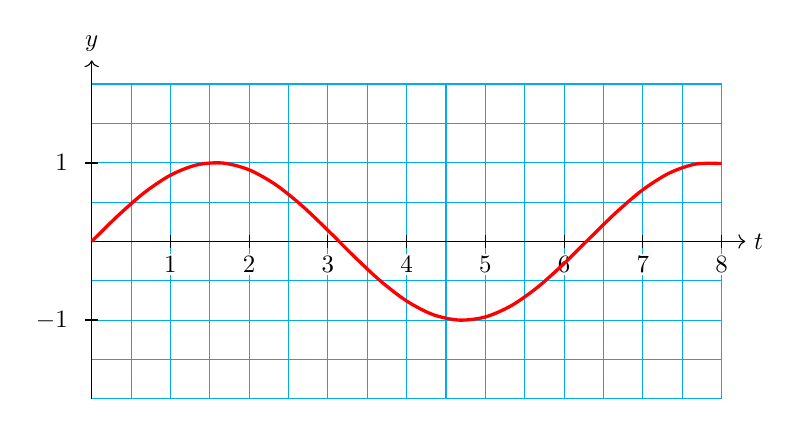
\begin{tikzpicture}

\draw[cyan,step=1/2] (0,-2) grid (8,2);
\draw[->] (0,0) -- (8.3,0) node[right, scale=0.9] {$t$};
\draw[->] (0,-2) -- (0,2.3) node[above, scale=0.9] {$y$};

\foreach \x in {1,2, ...,8}
 \draw[black] (\x, .08) --++(0,-.16) node[below, fill=white, inner sep=1, yshift=-2, scale=0.9]{$\x$};
\foreach \y in {-1,1}
 \draw[black, thick] (.08,\y ) --++(-.16,0) node[anchor=east, xshift=-3, scale=0.9] {$\y$};

\draw[domain=0:8,smooth,variable=\x,red,very thick] plot ({\x},{sin(deg(\x))});

\end{tikzpicture}
\newline


exam6-3-1
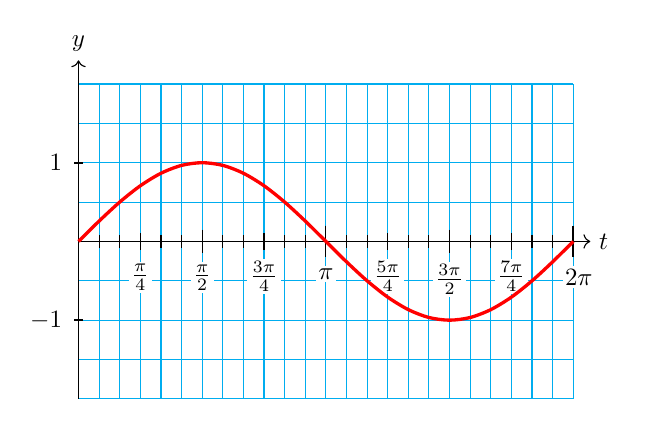
\begin{tikzpicture} [xscale=1]

\draw[cyan,xstep=pi/12, ystep=1/2] (0,-2) grid ($2*pi*(1,0)+(0,2) $);
\draw[->] (0,0) -- (6.5,0) node[right, scale=0.9] {$t$};
\draw[->] (0,-2) -- (0,2.3) node[above, scale=0.9] {$y$};

\foreach \x in {1, 2,...,24}
\draw[black] ($ pi*\x /12*(1,0) +(0,.08) $) --++(0,-.16);

\foreach \y in {-1,1}
\draw[black, thick] (.06,\y ) --++(-.12,0) node[anchor=east, xshift=-3, fill=white, inner sep=1pt, scale=.9] {$\y$};

\draw[black, thick] (2*pi,.2) --++(0,-.4) node[anchor=north, xshift=2,yshift=-3, fill=white, inner sep=1pt, scale=.9] {$2\pi$};

\draw[black] (pi,.2) --++(0,-.4) node[anchor=north, yshift=-3, fill=white, inner sep=1pt, scale=.9] {$\pi$};

\draw[black] (pi,.2) --++(0,-.4) node[anchor=north, yshift=-3, fill=white, inner sep=1pt, scale=.9] {$\pi$};

\draw[black] (pi/2,.15) --++(0,-.3) node[anchor=north, yshift=-3, fill=white, inner sep=1pt, scale=.9] {$\frac{\pi}{2}$};
\draw[black] (3*pi/2,.15) --++(0,-.3) node[anchor=north, yshift=-3, fill=white, inner sep=1pt, scale=.9] {$\frac{3\pi}{2}$};

\draw[black] (pi/4,.11) --++(0,-.22) node[anchor=north, yshift=-4, fill=white, inner sep=1pt, scale=.9] {$\frac{\pi}{4}$};

\draw[black] (3*pi/4,.11) --++(0,-.22) node[anchor=north, yshift=-3, fill=white, inner sep=1pt, scale=.9] {$\frac{3\pi}{4}$};
\draw[black] (5*pi/4,.11) --++(0,-.22) node[anchor=north, yshift=-3, fill=white, inner sep=1pt, scale=.9] {$\frac{5\pi}{4}$};
\draw[black] (7*pi/4,.11) --++(0,-.22) node[anchor=north, yshift=-3, fill=white, inner sep=1pt, scale=.9] {$\frac{7\pi}{4}$};

\draw[domain=0:2*pi,smooth,variable=\x,red,very thick] plot ({\x},{sin(deg(\x))});

\end{tikzpicture}
\newline


exer6-3-1
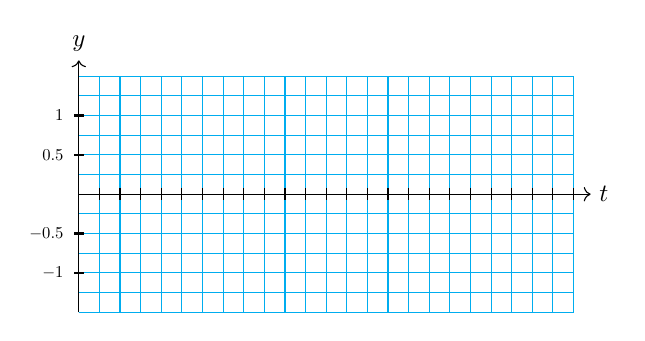
\begin{tikzpicture} 

\draw[cyan,xstep=pi/12, ystep=1/4] (0,-3/2) grid ($2*pi*(1,0)+(0,3/2) $);
\draw[->] (0,0) -- (6.5,0) node[right, scale=0.9] {$t$};
\draw[->] (0,-3/2) -- (0,1.7) node[above, scale=0.9] {$y$};

\foreach \x in {1, 2,...,24}
\draw[black] ($ pi*\x /12*(1,0) +(0,.08) $) --++(0,-.16);

\foreach \y in {-1, -0.5, 0.5,1}
\draw[black, thick] (.06,\y ) --++(-.12,0) node[anchor=east, xshift=-3, fill=white, inner sep=1pt, scale=.6] {$\y$};

\end{tikzpicture}
\newline


exer6-3-1ans
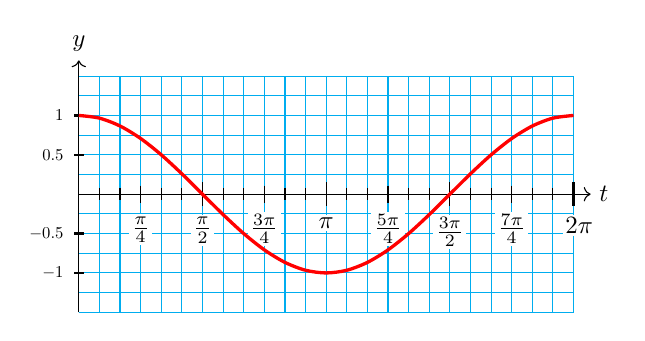
\begin{tikzpicture} 

\draw[cyan,xstep=pi/12, ystep=1/4] (0,-3/2) grid ($2*pi*(1,0)+(0,3/2) $);
\draw[->] (0,0) -- (6.5,0) node[right, scale=0.9] {$t$};
\draw[->] (0,-3/2) -- (0,1.7) node[above, scale=0.9] {$y$};

\foreach \x in {1, 2,...,24}
\draw[black] ($ pi*\x /12*(1,0) +(0,.08) $) --++(0,-.16);

\foreach \y in {-1, -0.5, 0.5,1}
\draw[black, thick] (.06,\y ) --++(-.12,0) node[anchor=east, xshift=-3, fill=white, inner sep=1pt, scale=.6] {$\y$};


\draw[black, thick] (2*pi,.15) --++(0,-.3) node[anchor=north, xshift=2,yshift=-3, fill=white, inner sep=1pt, scale=.9] {$2\pi$};

\draw[black] (pi,.15) --++(0,-.3) node[anchor=north, yshift=-3, fill=white, inner sep=1pt, scale=.9] {$\pi$};

\draw[black] (pi,.15) --++(0,-.3) node[anchor=north, yshift=-3, fill=white, inner sep=1pt, scale=.9] {$\pi$};

\draw[black] (pi/2,.15) --++(0,-.3) node[anchor=north, yshift=-3, fill=white, inner sep=1pt, scale=.9] {$\frac{\pi}{2}$};
\draw[black] (3*pi/2,.15) --++(0,-.3) node[anchor=north, yshift=-3, fill=white, inner sep=1pt, scale=.9] {$\frac{3\pi}{2}$};

\draw[black] (pi/4,.11) --++(0,-.22) node[anchor=north, yshift=-4, fill=white, inner sep=1pt, scale=.9] {$\frac{\pi}{4}$};

\draw[black] (3*pi/4,.11) --++(0,-.22) node[anchor=north, yshift=-3, fill=white, inner sep=1pt, scale=.9] {$\frac{3\pi}{4}$};
\draw[black] (5*pi/4,.11) --++(0,-.22) node[anchor=north, yshift=-3, fill=white, inner sep=1pt, scale=.9] {$\frac{5\pi}{4}$};
\draw[black] (7*pi/4,.11) --++(0,-.22) node[anchor=north, yshift=-3, fill=white, inner sep=1pt, scale=.9] {$\frac{7\pi}{4}$};

\draw[domain=0:2*pi,smooth,variable=\x,red,very thick] plot ({\x},{cos(deg(\x))});

\end{tikzpicture}
\newline


fig-6-3-empty
\begin{tikzpicture} 

\draw[->] (0,0) -- (6.3,0) ;
\draw[->] (0,-2) -- (0,2.3);

\foreach \x in {1.5, 3, 4.5, 6}
\draw[black] ($ \x *(1,0) +(0,.08) $) --++(0,-.16);

\foreach \y in {-2, -1, 1, 2}
\draw[black, thick] (.06,\y ) --++(-.12,0) node[anchor=east, xshift=-3, fill=white, inner sep=1pt, scale=.9] {$\y$};

\end{tikzpicture}
\newline



act6-2

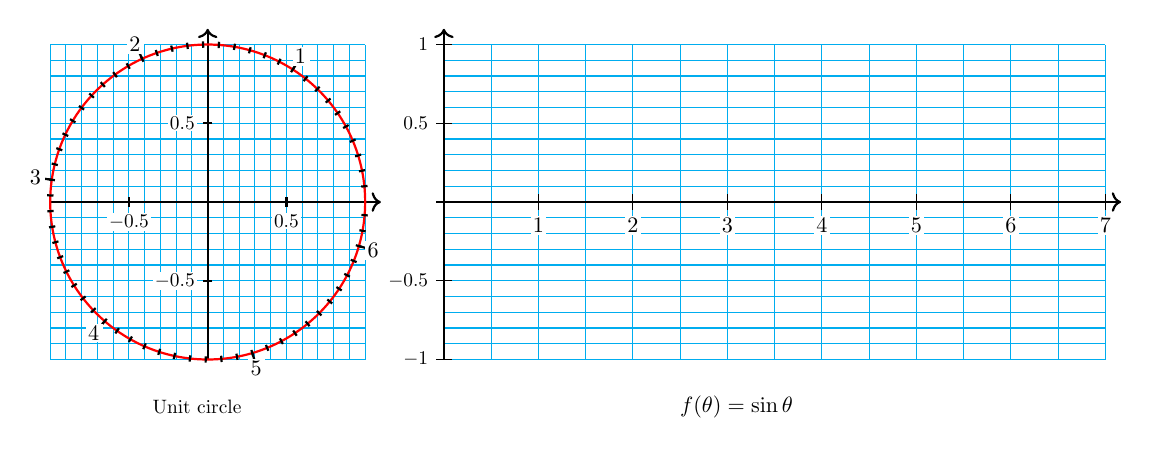
\begin{tikzpicture} [scale=2]

\draw[cyan] (-1.0001,-1.0001) grid[step = 0.1] (1,1);
\draw[black, thick, ->] (-1,0)--(1.1,0);
\draw[black, thick, ->] (0,-1)--(0,1.1);

\draw[red,thick] (0,0) circle (1cm);

\foreach \i in {0.1, 0.2, ..., 6.2} {
 \draw[black, thick] ({deg(\i)}:.98) -- ({deg(\i)}:1.02);
};
\foreach \i in {1,2, ..., 6} {
 \draw[black, thick] ({deg(\i)}:1) -- ({deg(\i)}:1.05);
 \node[text width=.2cm, fill=white, inner sep=1, scale=.8] at ({deg(\i)}:1.1) { $\i$};
};
\foreach \i in {-0.5, 0.5} {
 \draw[black, thick] (0.03,\i) -- (-0.03,\i) node[left, xshift=-2, fill=white, inner sep=1, scale=.7]{ $\i$};
 \draw[black, thick] (\i,0.03) -- (\i,-0.03) node[below, yshift=-2, fill=white, inner sep=1, scale=.7]{$\i$};
};

\node[text width=2cm, scale=.7] at (0,-1.3) {Unit circle};

%second grid
\draw[cyan] (1.4999,-1.0001) grid[xstep=.3, ystep=.1] (5.7,1);
\draw[black,thick,->] (1.45,0)--(5.8,0);
\draw[black,thick,->] (1.5,-1)--(1.5,1.1);

\foreach \x [evaluate=\x as \xi using (1.5 + .6* \x )]  in {1, 2,...,7}
 \draw[black] (\xi,.05)--++(0,-.1) node[below, yshift=-2, fill=white, inner sep =1, scale=.8] {$\x$};
 \foreach \y in {-1, -0.5, 0.5,1}
  \draw[black] (1.55,\y)--++(-.1,0) node[left, xshift=-2, fill=white, inner sep =1, scale=.7] {$\y$};

\node[text width=3cm, scale=.8] at (3.6,-1.3) {$ f(\theta) =\sin \theta $};

\end{tikzpicture}
\newline





act6-3

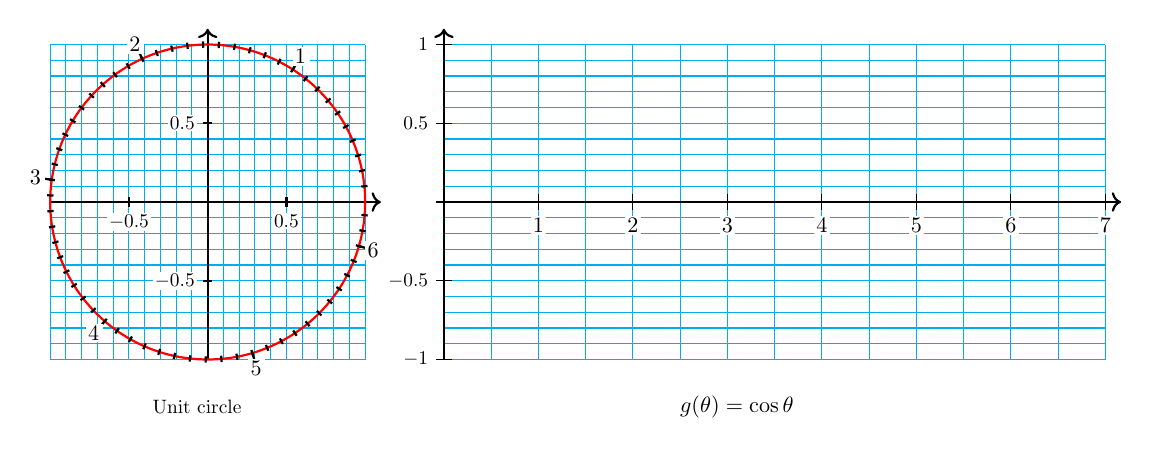
\begin{tikzpicture} [scale=2]

\draw[cyan] (-1.0001,-1.0001) grid[step = 0.1] (1,1);
\draw[black, thick, ->] (-1,0)--(1.1,0);
\draw[black, thick, ->] (0,-1)--(0,1.1);

\draw[red,thick] (0,0) circle (1cm);

\foreach \i in {0.1, 0.2, ..., 6.2} {
 \draw[black, thick] ({deg(\i)}:.98) -- ({deg(\i)}:1.02);
};
\foreach \i in {1,2, ..., 6} {
 \draw[black, thick] ({deg(\i)}:1) -- ({deg(\i)}:1.05);
 \node[text width=.2cm, fill=white, inner sep=1, scale=.8] at ({deg(\i)}:1.1) { $\i$};
};
\foreach \i in {-0.5, 0.5} {
 \draw[black, thick] (0.03,\i) -- (-0.03,\i) node[left, xshift=-2, fill=white, inner sep=1, scale=.7]{ $\i$};
 \draw[black, thick] (\i,0.03) -- (\i,-0.03) node[below, yshift=-2, fill=white, inner sep=1, scale=.7]{$\i$};
};

\node[text width=2cm, scale=.7] at (0,-1.3) {Unit circle};

%second grid
\draw[cyan] (1.4999,-1.0001) grid[xstep=.3, ystep=.1] (5.7,1);
\draw[black,thick,->] (1.45,0)--(5.8,0);
\draw[black,thick,->] (1.5,-1)--(1.5,1.1);

\foreach \x [evaluate=\x as \xi using (1.5 + .6* \x )]  in {1, 2,...,7}
 \draw[black] (\xi,.05)--++(0,-.1) node[below, yshift=-2, fill=white, inner sep =1, scale=.8] {$\x$};
 \foreach \y in {-1, -0.5, 0.5,1}
  \draw[black] (1.55,\y)--++(-.1,0) node[left, xshift=-2, fill=white, inner sep =1, scale=.7] {$\y$};

\node[text width=3cm, scale=.8] at (3.6,-1.3) {$ g(\theta) =\cos \theta $};

\end{tikzpicture}
\newline


exam6-3-2 tangent graph
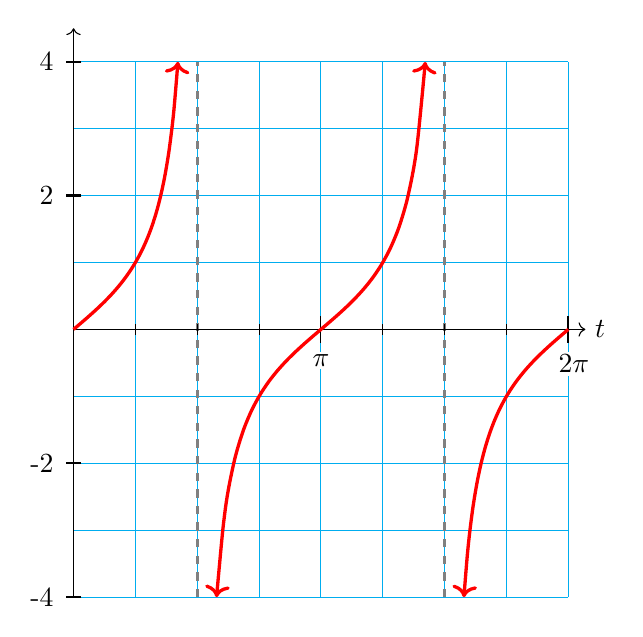
\begin{tikzpicture} [yscale=0.85]

\draw[cyan,xstep=pi/4,ystep=1]
(0,-4) grid (2*pi,4);

\draw[gray, very thick, dashed] (pi/2,-4)--++(0,8);
\draw[gray, very thick, dashed] (3*pi/2,-4)--++(0,8);

\draw[->] (-0,0) -- (6.5,0) node[right] {$t$};
\draw[->] (0,-4) -- (0,4.5) ;

\foreach \x in {1,2,...,8}
\draw[black] ($ pi*\x /4*(1,0) +(0,.08) $) --++(0,-.16);
\foreach \y in {-4,-2,2, 4}
\draw[black, thick] (.10,\y ) --++(-.2,0) node[anchor=east, xshift=-3, fill=white, inner sep=1pt] {\y};

\draw[black, thick] (2*pi,.2) --++(0,-.4) node[anchor=north, xshift=2,yshift=-3, fill=white, inner sep=1pt] {$2\pi$};

\draw[black] (pi,.2) --++(0,-.4) node[anchor=north, yshift=-3, fill=white, inner sep=1pt] {$\pi$};

\draw[domain={pi-atan(4)*pi/180}:{pi+atan(4)*pi/180}, smooth, variable=\x,red,very thick, <->] plot ({\x},{tan(deg(\x))}) ;

\draw[domain={0:atan(4)*pi/180}, smooth, variable=\x,red,very thick,->] plot ({\x},{tan(deg(\x))}) ;
\draw[domain={2*pi-atan(4)*pi/180:2*pi}, smooth, variable=\x,red,very thick, <-] plot ({\x},{tan(deg(\x))}) ;

\end{tikzpicture}
\newline



exer6-3-2

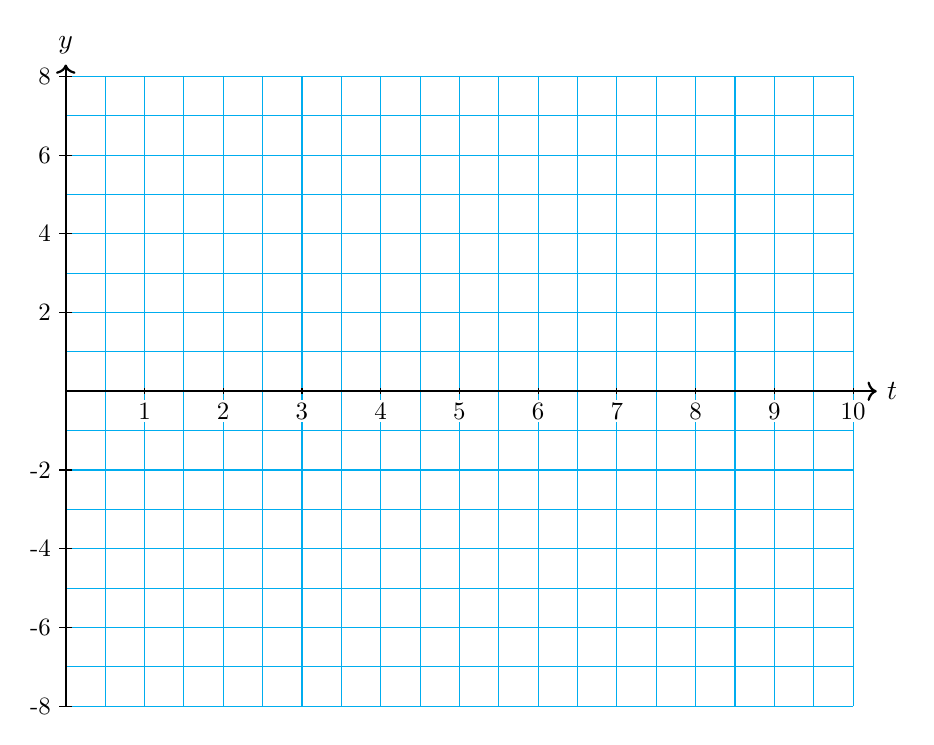
\begin{tikzpicture} [yscale=0.5]

\draw[cyan] (0,-8) grid[xstep=0.5, ystep=1] (10,8);
\draw[black,thick,->] (0,0)--(10.3,0) node[right]{$t$};
\draw[black,thick,->](0,-8)--(0,8.3) node[above] {$y$};

\foreach \x in {1,2,...,10} \draw[black] (\x,0.08)--++(0,-.16) node[below, yshift=-2, fill=white, inner sep=1, scale=0.9] {\x};
\foreach \y in {-8, -6, -4, -2, 2, 4, 6, 8} \draw[black] (0.08,\y)--++(-.16,0) node[left, xshift=-2, fill=white, inner sep=1, scale=0.9] {\y};

\end{tikzpicture};
\newline



exer6-3-2ans

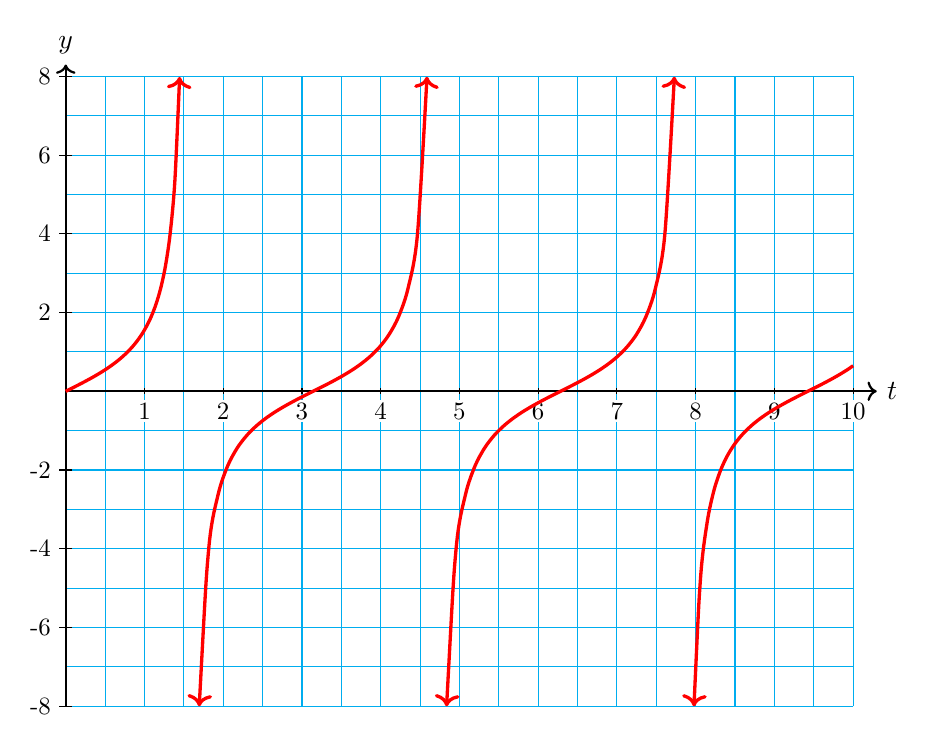
\begin{tikzpicture} [yscale=0.5]

\draw[cyan] (0,-8) grid[xstep=0.5, ystep=1] (10,8);
\draw[black,thick,->] (0,0)--(10.3,0) node[right]{$t$};
\draw[black,thick,->](0,-8)--(0,8.3) node[above] {$y$};

\foreach \x in {1,2,...,10} \draw[black] (\x,0.08)--++(0,-.16) node[below, yshift=-2, fill=white, inner sep=1, scale=0.9] {\x};
\foreach \y in {-8, -6, -4, -2, 2, 4, 6, 8} \draw[black] (0.08,\y)--++(-.16,0) node[left, xshift=-2, fill=white, inner sep=1, scale=0.9] {\y};

\draw[domain={pi-atan(8)*pi/180}:{pi+atan(8)*pi/180}, smooth, variable=\x,red,very thick, <->] plot ({\x},{tan(deg(\x))}) ;
\draw[domain={2*pi-atan(8)*pi/180}:{2*pi+atan(8)*pi/180}, smooth, variable=\x,red,very thick, <->] plot ({\x},{tan(deg(\x))}) ;

\draw[domain={0:atan(8)*pi/180}, smooth, variable=\x,red,very thick,->] plot ({\x},{tan(deg(\x))}) ;
\draw[domain={3*pi-atan(8)*pi/180:10}, smooth, variable=\x,red,very thick, <-] plot ({\x},{tan(deg(\x))}) ;


\end{tikzpicture};
\newline



act6-4

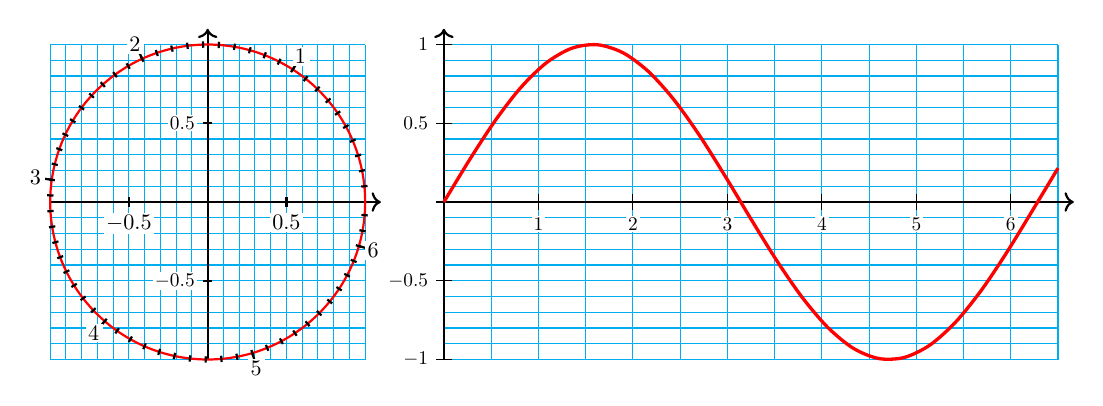
\begin{tikzpicture} [scale=2]

\draw[cyan] (-1.0001,-1.0001) grid[step = 0.1] (1,1);
\draw[black, thick, ->] (-1,0)--(1.1,0);
\draw[black, thick, ->] (0,-1)--(0,1.1);

\draw[red,thick] (0,0) circle (1cm);

\foreach \i in {0.1, 0.2, ..., 6.2} {
 \draw[black, thick] ({deg(\i)}:.98) -- ({deg(\i)}:1.02);
};
\foreach \i in {1,2, ..., 6} {
 \draw[black, thick] ({deg(\i)}:1) -- ({deg(\i)}:1.05);
 \node[text width=.2cm, fill=white, inner sep=1, scale=.8] at ({deg(\i)}:1.1) { $\i$};
};
\foreach \i in {-0.5, 0.5} {
 \draw[black, thick] (0.03,\i) -- (-0.03,\i) node[left, xshift=-2, fill=white, inner sep=1, scale=.7]{ $\i$};
 \draw[black, thick] (\i,0.03) -- (\i,-0.03) node[below, yshift=-2, fill=white, inner sep=1, scale=.8]{$\i$};
};


%second grid
\draw[cyan] (1.4999,-1.0001) grid[xstep=.3, ystep=.1] (5.4,1);
\draw[black,thick,->] (1.45,0)--(5.5,0);
\draw[black,thick,->] (1.5,-1)--(1.5,1.1);

\foreach \x [evaluate=\x as \xi using (1.5 + .6* \x )]  in {1, 2,...,6}
 \draw[black] (\xi,.05)--++(0,-.1) node[below, yshift=-2, fill=white, inner sep =1, scale=.7] {$\x$};
 \foreach \y in {-1, -0.5, 0.5,1}
  \draw[black] (1.55,\y)--++(-.1,0) node[left, xshift=-2, fill=white, inner sep =1, scale=.7] {$\y$};

\draw[domain=1.5:5.4,smooth,variable=\x,red,very thick] plot ({\x},{ sin(deg( (\x-1.5)/.6))});

\end{tikzpicture}
\newline



act6-5

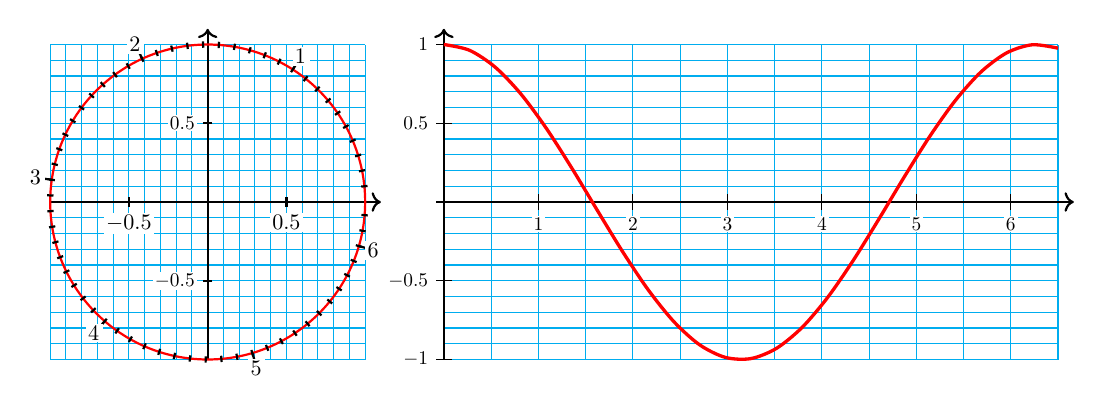
\begin{tikzpicture} [scale=2]

\draw[cyan] (-1.0001,-1.0001) grid[step = 0.1] (1,1);
\draw[black, thick, ->] (-1,0)--(1.1,0);
\draw[black, thick, ->] (0,-1)--(0,1.1);

\draw[red,thick] (0,0) circle (1cm);

\foreach \i in {0.1, 0.2, ..., 6.2} {
 \draw[black, thick] ({deg(\i)}:.98) -- ({deg(\i)}:1.02);
};
\foreach \i in {1,2, ..., 6} {
 \draw[black, thick] ({deg(\i)}:1) -- ({deg(\i)}:1.05);
 \node[text width=.2cm, fill=white, inner sep=1, scale=.8] at ({deg(\i)}:1.1) { $\i$};
};
\foreach \i in {-0.5, 0.5} {
 \draw[black, thick] (0.03,\i) -- (-0.03,\i) node[left, xshift=-2, fill=white, inner sep=1, scale=.7]{ $\i$};
 \draw[black, thick] (\i,0.03) -- (\i,-0.03) node[below, yshift=-2, fill=white, inner sep=1, scale=.8]{$\i$};
};


%second grid
\draw[cyan] (1.4999,-1.0001) grid[xstep=.3, ystep=.1] (5.4,1);
\draw[black,thick,->] (1.45,0)--(5.5,0);
\draw[black,thick,->] (1.5,-1)--(1.5,1.1);

\foreach \x [evaluate=\x as \xi using (1.5 + .6* \x )]  in {1, 2,...,6}
 \draw[black] (\xi,.05)--++(0,-.1) node[below, yshift=-2, fill=white, inner sep =1, scale=.7] {$\x$};
 \foreach \y in {-1, -0.5, 0.5,1}
  \draw[black] (1.55,\y)--++(-.1,0) node[left, xshift=-2, fill=white, inner sep =1, scale=.7] {$\y$};

\draw[domain=1.5:5.4,smooth,variable=\x,red,very thick] plot ({\x},{ cos(deg( (\x-1.5)/.6))});

\end{tikzpicture}
\newline



exam6-3-3 cosine graph

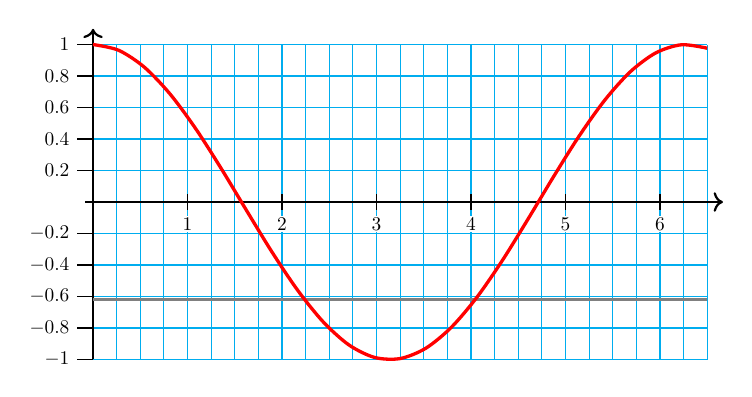
\begin{tikzpicture} [scale=2]

\draw[cyan] (0,-1.0001) grid[xstep=.15, ystep=.2] (3.9,1);
\draw[black,thick,->] (-0.05,0)--(4,0);
\draw[black,thick,->] (0,-1)--(0,1.1);

\foreach \x [evaluate=\x as \xi using ( .6* \x )]  in {1, 2,...,6}
 \draw[black] (\xi,.05)--++(0,-.1) node[below, yshift=-2, fill=white, inner sep =1, scale=.7] {$\x$};
 \foreach \y in {-1, -0.8,-0.6,-0.4,-0.2,0.2,0.4,0.6,0.8,1}
  \draw[black] (0,\y)--++(-.1,0) node[left, xshift=-2, fill=white, inner sep =1, scale=.7] {$\y$};

\draw[gray, very thick] (0,-0.62)--++(3.9,0);
\draw[domain=0:3.9,smooth,variable=\x,red,very thick] plot ({\x},{ cos(deg( (\x)/.6))});

\end{tikzpicture}
\newline



exam6-3-4 unit circle
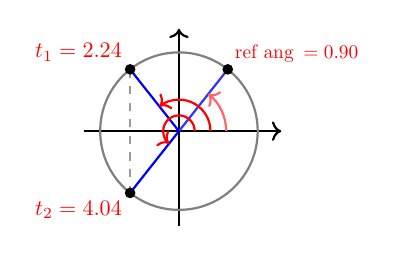
\begin{tikzpicture}

\coordinate (O) at (0,0);
\coordinate (A) at ({acos(0.62)}:1);
\coordinate (B) at ({acos(-0.62)}:1);
\coordinate (C) at ({180+acos(0.62)}:1);

\draw[black,thick,->] (-1.2,0) --++(2.5,0);
\draw[black,thick,->] (0,-1.2)--++(0,2.5);
\draw[gray,thick] (O) circle (1cm);

\draw[blue!80, thick] (O)--(A) node[above right, scale=0.7] {\color{red} ref ang $\,=0.90$};
\draw[blue, thick] (O)--(B) node[above left, scale=0.8] {\color{red} $t_1=2.24$};
\draw[blue, thick] (O)--(C) node[below left, scale=0.8] {\color{red} $t_2=4.04$};
\draw[gray!80,thick, dashed] (B)--(C);

\draw[red,thick,->] (.2,0) arc(0:{180+acos(0.62)}:0.2);
\draw[red,thick,->] (0.4,0) arc(0:{acos(-0.62)}:0.4);
\draw[red!60,thick,->] (0.6,0) arc(0:{acos(0.62)}:0.6);

\filldraw[black] (A) circle (0.06cm);
\filldraw[black] (B) circle (0.06cm);
\filldraw[black] (C) circle (0.06cm);

\end{tikzpicture}
\newline


fig-6-3-height 

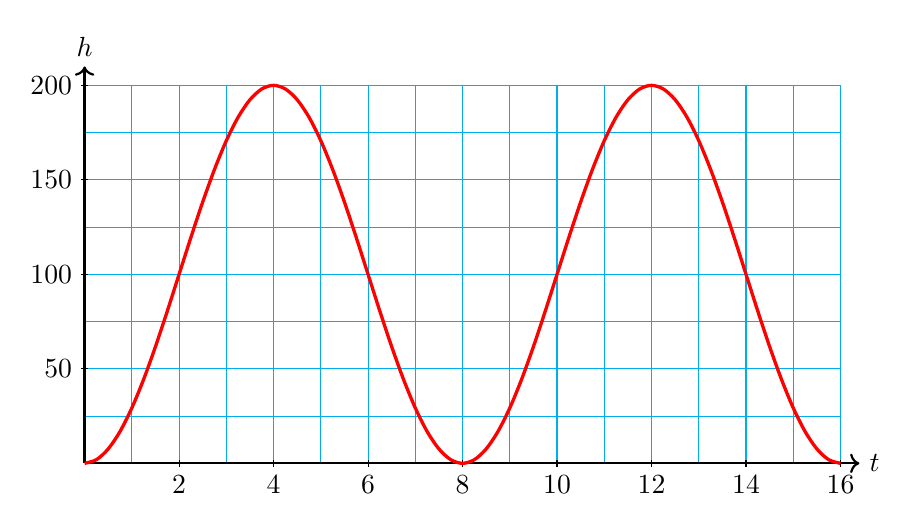
\begin{tikzpicture} [xscale=.6, yscale=.024]

\draw[cyan] (0,0) grid[ystep=25] (16,200);
\draw[black,thick,->] (0,0)--(16.4,0) node[right]{ $t$};
\draw[black,thick,->] (0,0)--(0,210) node[above]{ $h$};

\foreach \x in {2,4,..., 16} \draw[black] (\x,2)--++(0,-4) node[below, yshift=-2, fill=white, inner sep=1]{\x};
\foreach \y in {50, 100, 150, 200} \draw[black] (.08,\y)--++(-0.16,0) node[left, xshift=-2, fill=white, inner sep=1]{\y};

\draw[samples=65,domain=0:16,smooth,variable=\x,red,very thick] plot ({\x},{100-100* cos( 45*\x)});

\end{tikzpicture}
\newline



exam6-3-6
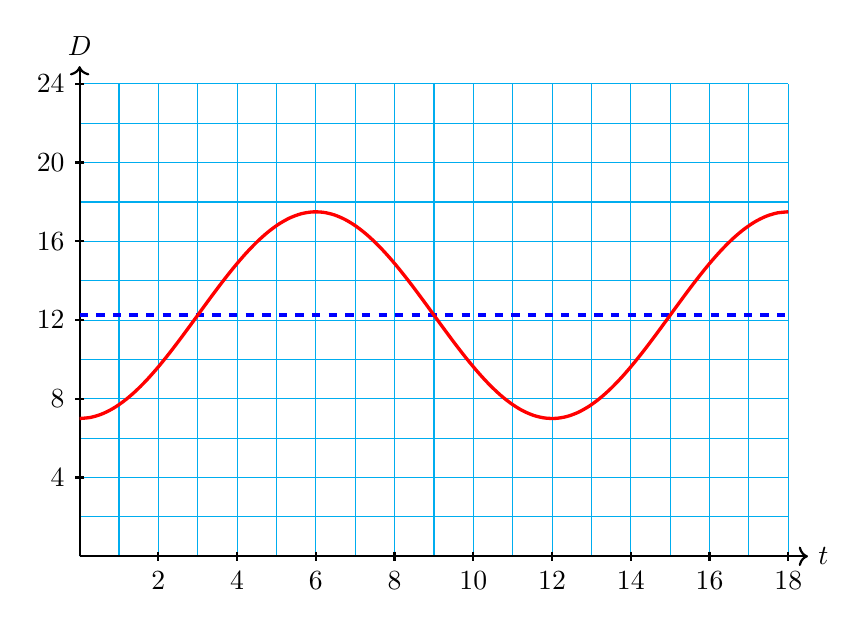
\begin{tikzpicture} [xscale=.5, yscale=.25]
\draw[cyan] (0,0) grid[ystep=2] (18,24);

\draw[black,thick,->] (0,0)--(18.5,0) node[right]{$t$};
\draw[black,thick,->] (0,0)--(0,24.9) node[above]{$D$};
\foreach \x in {2,4,...,18} \draw[black,thick] (\x,0.24)--++(0,-.48) node[below] {\x};
\foreach \y in {4,8,...,24} \draw[black,thick] (0.12,\y)--++(-.24,0) node[left] {\y};

\draw[blue, very thick, dashed] (0,12.25)--++(18,0);
\draw[samples=65,domain=0:18,smooth,variable=\x,red,very thick] plot ({\x},{12.25-5.25* cos( 30*\x)});

\end{tikzpicture}
\newline



exer6-3-6ans
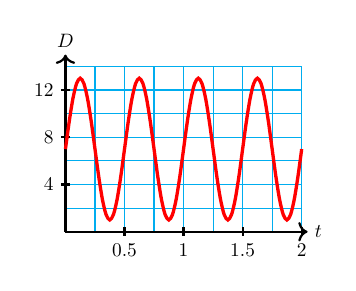
\begin{tikzpicture} [xscale=1.5, yscale=.15]
\draw[cyan] (0,0) grid[xstep=.25, ystep=2] (2,14);

\draw[black,thick,->] (0,0)--(2.05,0) node[right, scale=.7]{$t$};
\draw[black,thick,->] (0,0)--(0,15) node[above, scale=.7]{$D$};
\foreach \x in {0.5, 1, 1.5, 2} \draw[black,thick] (\x,0.4)--++(0,-.8) node[below, scale=.7] {\x};
\foreach \y in {4,8, 12} \draw[black,thick] (0.04,\y)--++(-.08,0) node[left, scale=.7] {\y};

\draw[samples=65,domain=0:2,smooth,variable=\x,red,very thick] plot ({\x},{7+6* sin( 4*180*\x)});

\end{tikzpicture}
\newline


fig-6-3-domrge

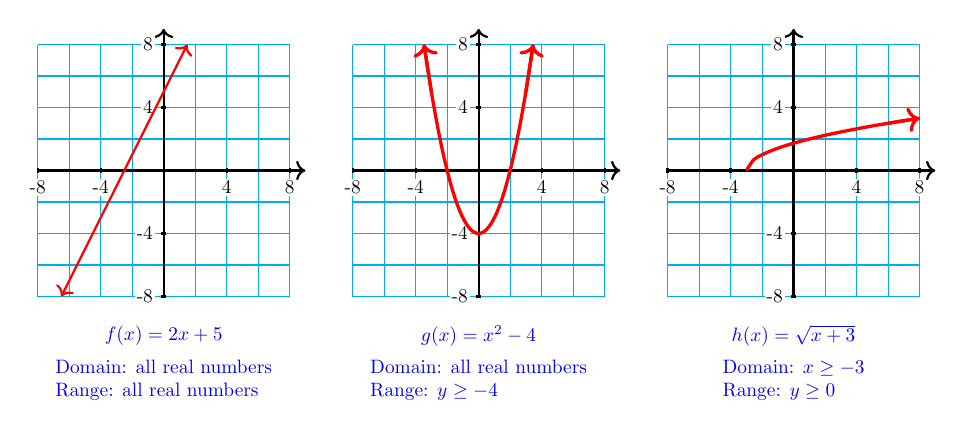
\begin{tikzpicture} [scale=.2]

\coordinate (O) at (0,0);
\coordinate (A) at (-8.001,-8.01);
\coordinate (B) at (8,8);
\draw[cyan] (A) grid[step=2] (B);
\draw[black,thick,->] (-8,0)--++(17.,0) ;
\draw[black,thick,->] (0,-8)--++(0,17) ;
\foreach \i in {-8,-4,4,8} {
 \draw[black,thick] (\i,0.16)--++(0,-.32)node[below, yshift=-2, fill=white, inner sep=1, scale=.7]{\i};
 \draw[black,thick] (0.16,\i)--++(-.32,0)node[left, xshift=-2, fill=white, inner sep=1, scale=.7]{\i};
};
\draw[red,thick,<->] (-13/2, -8)--(3/2,8);

\node[align=center, text=blue, scale=.7] at (0, -10.5) {$f(x)=2x+5$};
\node[align=left, text=blue, scale=.7] at (0, -13.3) { Domain: all real numbers \\ Range: all real numbers};


%second grid
\coordinate (O) at (20,0);
\coordinate (A) at (11.999,-8.01);
\coordinate (B) at (28.001,8);
\draw[cyan] (A) grid[step=2] (B);
\draw[black,thick,->] (12,0)--++(17.,0) ;
\draw[black,thick,->] (20,-8)--++(0,17) ;

\foreach \i [evaluate=\i as \ix using int(\i+20]  in {-8,-4,4,8} {
 \draw[black,thick] (\ix,0.16)--++(0,-.32)node[below, yshift=-2, fill=white, inner sep=1, scale=.7]{\i};
 \draw[black,thick] (20.16,\i)--++(-.32,0)node[left, xshift=-2, fill=white, inner sep=1, scale=.7]{\i};
};

\draw[domain=16.536:23.4641,smooth,variable=\x,red,very thick] plot ({\x},{(\x-20)^2 -4});
\draw[red,very thick,<-] (16.536,8)--(17,5);
\draw[red,very thick,<-] (23.4641,8)--(23,5);

\node[align=center, text=blue, scale=.7] at (20, -10.5) {$g(x)=x^2-4$};
\node[align=left, text=blue, scale=.7] at (20, -13.3) { Domain: all real numbers \\ Range: $y \ge -4$};


%third grid
\coordinate (O) at (40,0);
\coordinate (A) at (31.999,-8.01);
\coordinate (B) at (48.001,8);
\draw[cyan] (A) grid[step=2] (B);
\draw[black,thick,->] (32,0)--++(17.,0) ;
\draw[black,thick,->] (40,-8)--++(0,17) ;

\foreach \i [evaluate=\i as \ix using int(\i+40]  in {-8,-4,4,8} {
 \draw[black,thick] (\ix,0.16)--++(0,-.32)node[below, yshift=-2, fill=white, inner sep=1, scale=.7]{\i};
 \draw[black,thick] (40.16,\i)--++(-.32,0)node[left, xshift=-2, fill=white, inner sep=1, scale=.7]{\i};
};

\draw[domain=37:48,smooth,variable=\x,red,very thick] plot ({\x},{sqrt(\x -37)});
\draw[red,very thick,->] (46,3)--(48,3.3166);

\node[align=center, text=blue, scale=.7] at (40, -10.5) {$h(x)=\sqrt{x+3}$};
\node[align=left, text=blue, scale=.7] at (40, -13.3) { Domain: $x \ge -3$ \\ Range: $y \ge 0$};

\end{tikzpicture}
\newline



exam6-3-7a parabola
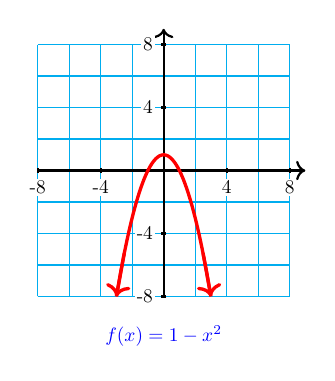
\begin{tikzpicture} [scale=.2]

\draw[cyan] (-8,-8) grid[step=2] (8,8);
\draw[black,thick,->] (-8,0)--++(17.,0) ;
\draw[black,thick,->] (0,-8)--++(0,17) ;
\foreach \i in {-8,-4,4,8} {
 \draw[black,thick] (\i,0.16)--++(0,-.32)node[below, yshift=-2, fill=white, inner sep=1, scale=.7]{\i};
 \draw[black,thick] (0.16,\i)--++(-.32,0)node[left, xshift=-2, fill=white, inner sep=1, scale=.7]{\i};
};
\draw[domain=-3:3,smooth,variable=\x,red,very thick] plot ({\x},{1-(\x) ^2});
\draw[red,very thick,->] (-5/2,-21/4)--(-3,-8);
\draw[red,very thick,->] (5/2,-21/4)--(3,-8);

\node[align=center, text=blue, scale=.7] at (0, -10.5) {$f(x)=1-x^2$};

\end{tikzpicture}
\newline



exam6-3-7b hyperbola
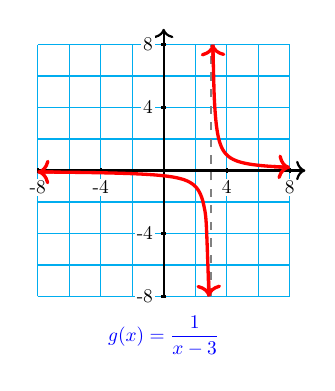
\begin{tikzpicture} [scale=.2]

\draw[cyan] (-8,-8) grid[step=2] (8,8);
\draw[black,thick,->] (-8,0)--++(17.,0) ;
\draw[black,thick,->] (0,-8)--++(0,17) ;
\foreach \i in {-8,-4,4,8} {
 \draw[black,thick] (\i,0.16)--++(0,-.32)node[below, yshift=-2, fill=white, inner sep=1, scale=.7]{\i};
 \draw[black,thick] (0.16,\i)--++(-.32,0)node[left, xshift=-2, fill=white, inner sep=1, scale=.7]{\i};
};

\draw[gray,thick,dashed] (3,-8)--(3,8);
\draw[samples=65,domain=-8:23/8,smooth,variable=\x,red,very thick] plot ({\x},{1/(\x -3)});
\draw[red,very thick,->] (-7,-1/10)--(-8,-1/11);
\draw[red,very thick,->] (20/7,-7)--(23/8,-8);

\draw[samples=65,domain=25/8:8,smooth,variable=\x,red,very thick] plot ({\x},{1/(\x -3)});
\draw[red,very thick,->] (22/7,7)--(25/8,8);
\draw[red,very thick,->] (7,1/4)--(8,1/5);
\node[align=center, text=blue, scale=.7] at (0, -10.5) {$\displaystyle g(x)=\frac{1}{x-3}$};

\end{tikzpicture}
\newline



fig-6-3-sumsin sine graph

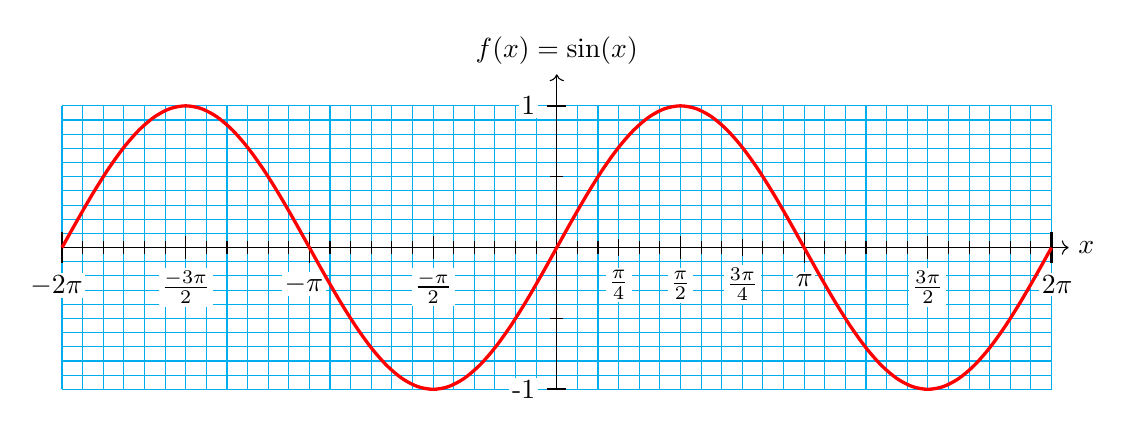
\begin{tikzpicture}

\draw[cyan,xstep=pi/12,ystep=0.18]
(-2*pi,-1.8) grid (2*pi,1.8);

\draw[->] (-6.3,0) -- (6.5,0) node[right] {$x$};
\draw[->] (0,-1.8) -- (0,2.2) node[above] {$f(x)=\sin(x)$};

\foreach \x in {-24,-23,...,24}
\draw[black] ($ pi*\x /12*(1,0) +(0,.08) $) --++(0,-.16);
\foreach \y in {-0.9, 0.9}
\draw[black] (.08,\y ) --++(-.16,0);
\foreach \y in {-1,1}
\draw[black, thick] (.12,1.8*\y ) --++(-.24,0) node[anchor=east, xshift=-3, fill=white, inner sep=1pt] {\y};

\draw[black, thick] (-2*pi,.2) --++(0,-.4) node[anchor=north, xshift=-2,yshift=-3, fill=white, inner sep=1pt] {$-2\pi$};
\draw[black, thick] (2*pi,.2) --++(0,-.4) node[anchor=north, xshift=2,yshift=-3, fill=white, inner sep=1pt] {$2\pi$};

\draw[black] (pi,.2) --++(0,-.4) node[anchor=north, yshift=-3, fill=white, inner sep=1pt] {$\pi$};

\draw[black] (pi,.2) --++(0,-.4) node[anchor=north, yshift=-3, fill=white, inner sep=1pt] {$\pi$};
\draw[black] (-pi,.2) --++(0,-.4) node[anchor=north, xshift=-2,yshift=-3, fill=white, inner sep=1pt] {$-\pi$};
\draw[black] (-pi/2,.15) --++(0,-.3) node[anchor=north, yshift=-3, fill=white, inner sep=1pt] {$\frac{-\pi}{2}$};
\draw[black] (pi/2,.15) --++(0,-.3) node[anchor=north, yshift=-3, fill=white, inner sep=1pt] {$\frac{\pi}{2}$};
\draw[black] (3*pi/2,.15) --++(0,-.3) node[anchor=north, yshift=-3, fill=white, inner sep=1pt] {$\frac{3\pi}{2}$};
\draw[black] (-3*pi/2,.15) --++(0,-.3) node[anchor=north, yshift=-3, fill=white, inner sep=1pt] {$\frac{-3\pi}{2}$};

\draw[black] (pi/4,.11) --++(0,-.22) node[anchor=north, yshift=-4, fill=white, inner sep=1pt] {$\frac{\pi}{4}$};

\draw[black] (3*pi/4,.11) --++(0,-.22) node[anchor=north, yshift=-3, fill=white, inner sep=1pt] {$\frac{3\pi}{4}$};

\draw[samples=65,domain=-2*pi:2*pi,smooth,variable=\x,red,very thick] plot ({\x},{1.8*sin(deg(\x))});

\end{tikzpicture}
\newline


fig-6-3-sumcos cosine graph

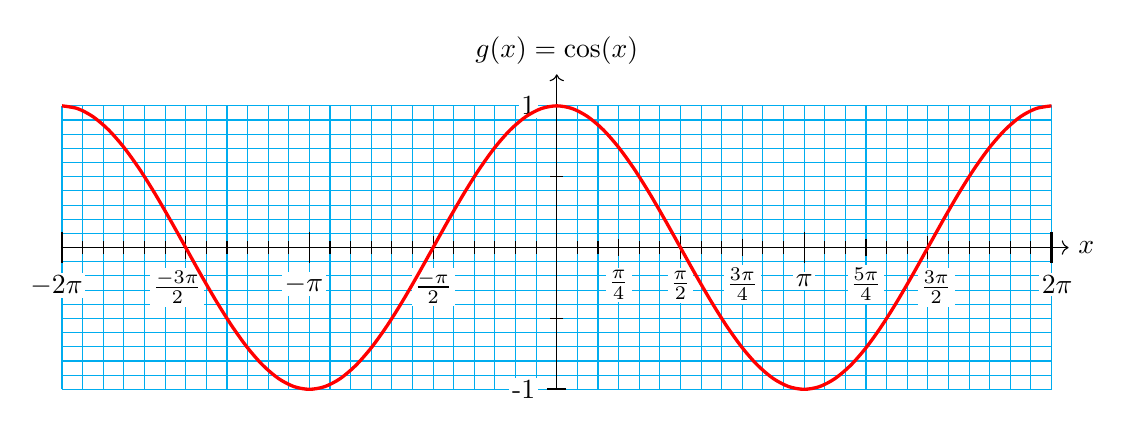
\begin{tikzpicture} 

\draw[cyan,xstep=pi/12,ystep=0.18]
(-2*pi,-1.8) grid (2*pi,1.8);

\draw[->] (-6.3,0) -- (6.5,0) node[right] {$x$};
\draw[->] (0,-1.8) -- (0,2.2) node[above] {$g(x)=\cos(x)$};

\foreach \x in {-24,-23,...,24}
\draw[black] ($ pi*\x /12*(1,0) +(0,.08) $) --++(0,-.16);
\foreach \y in {-0.9, 0.9}
\draw[black] (.08,\y ) --++(-.16,0);
\foreach \y in {-1,1}
\draw[black, thick] (.12,1.8*\y ) --++(-.24,0) node[anchor=east, xshift=-3, fill=white, inner sep=1pt] {\y};

\draw[black, thick] (-2*pi,.2) --++(0,-.4) node[anchor=north, xshift=-2,yshift=-3, fill=white, inner sep=1pt] {$-2\pi$};
\draw[black, thick] (2*pi,.2) --++(0,-.4) node[anchor=north, xshift=2,yshift=-3, fill=white, inner sep=1pt] {$2\pi$};

\draw[black] (pi,.2) --++(0,-.4) node[anchor=north, yshift=-3, fill=white, inner sep=1pt] {$\pi$};

\draw[black] (pi,.2) --++(0,-.4) node[anchor=north, yshift=-3, fill=white, inner sep=1pt] {$\pi$};
\draw[black] (-pi,.2) --++(0,-.4) node[anchor=north, xshift=-2,yshift=-3, fill=white, inner sep=1pt] {$-\pi$};
\draw[black] (-pi/2,.15) --++(0,-.3) node[anchor=north, yshift=-3, fill=white, inner sep=1pt] {$\frac{-\pi}{2}$};
\draw[black] (pi/2,.15) --++(0,-.3) node[anchor=north, yshift=-3, fill=white, inner sep=1pt] {$\frac{\pi}{2}$};
\draw[black] (3*pi/2,.15) --++(0,-.3) node[anchor=north,xshift=3, yshift=-3, fill=white, inner sep=1pt] {$\frac{3\pi}{2}$};
\draw[black] (-3*pi/2,.15) --++(0,-.3) node[anchor=north,xshift=-3, yshift=-3, fill=white, inner sep=1pt] {$\frac{-3\pi}{2}$};

\draw[black] (pi/4,.11) --++(0,-.22) node[anchor=north, yshift=-4, fill=white, inner sep=1pt] {$\frac{\pi}{4}$};

\draw[black] (3*pi/4,.11) --++(0,-.22) node[anchor=north, yshift=-3, fill=white, inner sep=1pt] {$\frac{3\pi}{4}$};

\draw[black] (5*pi/4,.11) --++(0,-.22) node[anchor=north, yshift=-3, fill=white, inner sep=1pt] {$\frac{5\pi}{4}$};

\draw[samples=65, domain=-2*pi:2*pi,smooth,variable=\x,red,very thick] plot ({\x},{1.8*cos(deg(\x))});

\end{tikzpicture}
\newline


fig-6-3-sumtan tangent graph

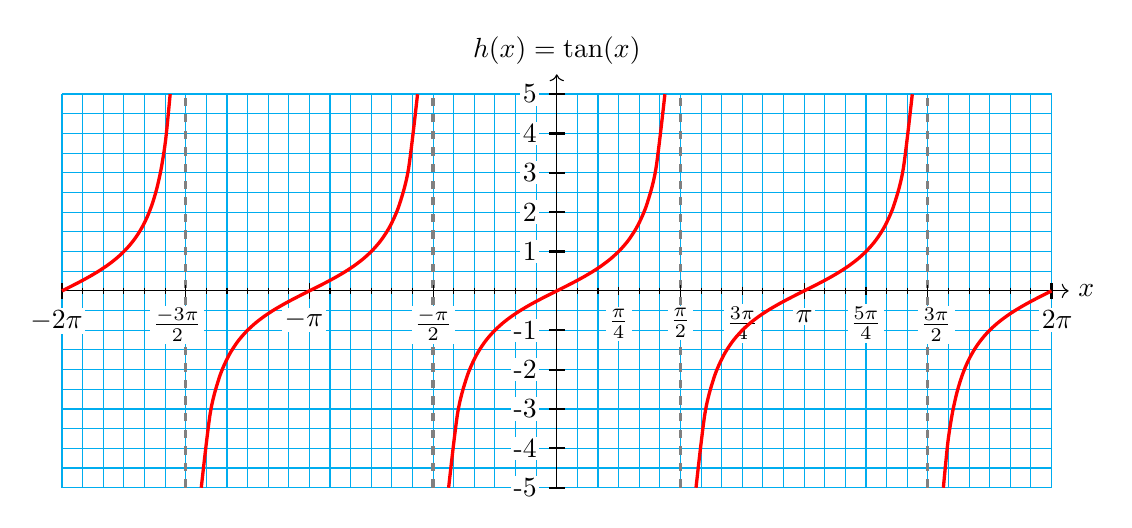
\begin{tikzpicture} [yscale=.5]

\draw[cyan,xstep=pi/12,ystep=0.5]
(-2*pi,-5) grid (2*pi,5);

\draw[->] (-6.3,0) -- (6.5,0) node[right] {$x$};
\draw[->] (0,-5) -- (0,5.5) node[above] {$h(x)=\tan(x)$};

\draw[gray, very thick,dashed] (-3*pi/2,-5)--++(0,10);
\draw[gray, very thick,dashed] (-pi/2,-5)--++(0,10);
\draw[gray, very thick,dashed] (pi/2,-5)--++(0,10);
\draw[gray, very thick,dashed] (3*pi/2,-5)--++(0,10);


\foreach \x in {-24,-23,...,24}
\draw[black] ($ pi*\x /12*(1,0) +(0,.08) $) --++(0,-.16);
\foreach \y in {-5,-4,...,-1,1,2,...,5}
\draw[black, thick] (.10,\y ) --++(-.2,0) node[anchor=east, xshift=-3, fill=white, inner sep=1pt] {\y};

\draw[black, thick] (-2*pi,.2) --++(0,-.4) node[anchor=north, xshift=-2,yshift=-3, fill=white, inner sep=1pt] {$-2\pi$};
\draw[black, thick] (2*pi,.2) --++(0,-.4) node[anchor=north, xshift=2,yshift=-3, fill=white, inner sep=1pt] {$2\pi$};

\draw[black] (pi,.2) --++(0,-.4) node[anchor=north, yshift=-3, fill=white, inner sep=1pt] {$\pi$};

\draw[black] (pi,.2) --++(0,-.4) node[anchor=north, yshift=-3, fill=white, inner sep=1pt] {$\pi$};
\draw[black] (-pi,.2) --++(0,-.4) node[anchor=north, xshift=-2,yshift=-3, fill=white, inner sep=1pt] {$-\pi$};
\draw[black] (-pi/2,.15) --++(0,-.3) node[anchor=north, yshift=-3, fill=white, inner sep=1pt] {$\frac{-\pi}{2}$};
\draw[black] (pi/2,.15) --++(0,-.3) node[anchor=north, yshift=-3, fill=white, inner sep=1pt] {$\frac{\pi}{2}$};
\draw[black] (3*pi/2,.15) --++(0,-.3) node[anchor=north,xshift=3, yshift=-3, fill=white, inner sep=1pt] {$\frac{3\pi}{2}$};
\draw[black] (-3*pi/2,.15) --++(0,-.3) node[anchor=north,xshift=-3, yshift=-3, fill=white, inner sep=1pt] {$\frac{-3\pi}{2}$};

\draw[black] (pi/4,.11) --++(0,-.22) node[anchor=north, yshift=-4, fill=white, inner sep=1pt] {$\frac{\pi}{4}$};

\draw[black] (3*pi/4,.11) --++(0,-.22) node[anchor=north, yshift=-3, fill=white, inner sep=1pt] {$\frac{3\pi}{4}$};

\draw[black] (5*pi/4,.11) --++(0,-.22) node[anchor=north, yshift=-3, fill=white, inner sep=1pt] {$\frac{5\pi}{4}$};

\foreach \i in {-1, 0, 1}
	\draw[domain={\i*pi-atan(5)*pi/180}:{\i*pi+atan(5)*pi/180}, smooth, variable=\x,red,very thick] plot ({\x},{tan(deg(\x))}) ;
	
\draw[domain={-2*pi:atan(5)*pi/180-2*pi}, smooth, variable=\x,red,very thick] plot ({\x},{tan(deg(\x))}) ;
\draw[domain={2*pi-atan(5)*pi/180:2*pi}, smooth, variable=\x,red,very thick] plot ({\x},{tan(deg(\x))}) ;

\end{tikzpicture}
\newline



fig-6-3-sq
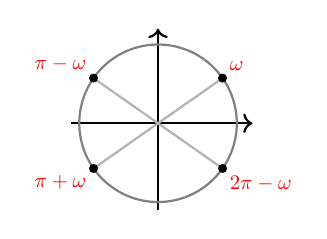
\begin{tikzpicture} 

\draw[black,thick,->] (-1.1,0)--(1.2,0);
\draw[black,thick,->] (0,-1.1)--(0,1.2);
\draw[gray,thick] (0,0) circle (1cm);

\coordinate(A) at (35:1);
\coordinate(B) at (145:1);
\coordinate(C) at (215:1);
\coordinate(D) at (325:1);

\draw[gray!60, thick] (A)--(C);
\draw[gray!60, thick] (B)--(D);

\filldraw[black] (A) circle (.05cm) node[above right, scale=.75, color=red]{$\omega$};;
\filldraw[black] (B) circle (.05cm) node[above left, scale=.75, color=red]{$\pi -\omega$};;
\filldraw[black] (C) circle (.05cm) node[below left, scale=.75, color=red]{$\pi +\omega$};;
\filldraw[black] (D) circle (.05cm) node[below right, scale=.75, color=red]{$2\pi-\omega$};;

\end{tikzpicture}
\newline


hp6-3-1 grid

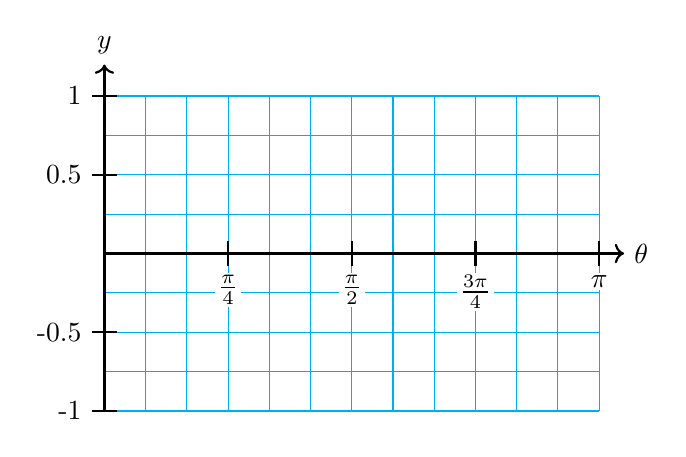
\begin{tikzpicture} [scale=2]
\draw[cyan] (0,-1) grid[xstep=pi/12, ystep=1/4] (pi,1);
\draw[black,thick, ->] (0,0) --(3.3,0) node[right] {$\theta$};
\draw[black,thick,->] (0,-1)--(0,1.2) node[above]{$y$};
\foreach \y in {-1,-0.5, 0.5, 1} \draw[black,thick] (.08,\y)--++(-.16,0) node[left]{\y};

\draw[black,thick] (pi/4,.08)--++(0,-.16) node[below, yshift=-2, fill=white, inner sep=1] {$\frac{\pi}{4}$};
\draw[black,thick] (pi/2,.08)--++(0,-.16) node[below, yshift=-2, fill=white, inner sep=1] {$\frac{\pi}{2}$};
\draw[black,thick] (3*pi/4,.08)--++(0,-.16) node[below, yshift=-2, fill=white, inner sep=1] {$\frac{3\pi}{4}$};
\draw[black,thick] (pi,.08)--++(0,-.16) node[below, yshift=-2, fill=white, inner sep=1] {$\pi$};

\end{tikzpicture}
\newline



hp6-3-1ans cosine

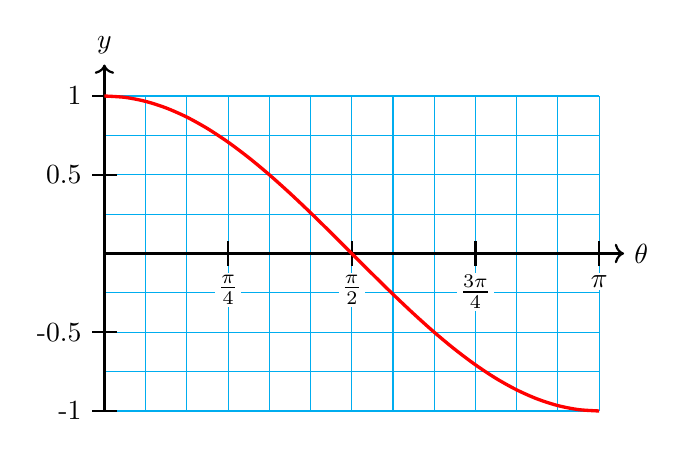
\begin{tikzpicture} [scale=2]
\draw[cyan] (0,-1) grid[xstep=pi/12, ystep=1/4] (pi,1);
\draw[black,thick, ->] (0,0) --(3.3,0) node[right] {$\theta$};
\draw[black,thick,->] (0,-1)--(0,1.2) node[above]{$y$};
\foreach \y in {-1,-0.5, 0.5, 1} \draw[black,thick] (.08,\y)--++(-.16,0) node[left]{\y};

\draw[black,thick] (pi/4,.08)--++(0,-.16) node[below, yshift=-2, fill=white, inner sep=1] {$\frac{\pi}{4}$};
\draw[black,thick] (pi/2,.08)--++(0,-.16) node[below, yshift=-2, fill=white, inner sep=1] {$\frac{\pi}{2}$};
\draw[black,thick] (3*pi/4,.08)--++(0,-.16) node[below, yshift=-2, fill=white, inner sep=1] {$\frac{3\pi}{4}$};
\draw[black,thick] (pi,.08)--++(0,-.16) node[below, yshift=-2, fill=white, inner sep=1] {$\pi$};

\draw[domain=0:pi,smooth,variable=\x,red,very thick] plot ({\x},{cos(deg(\x))});

\end{tikzpicture}
\newline


hp6-3-3 grid

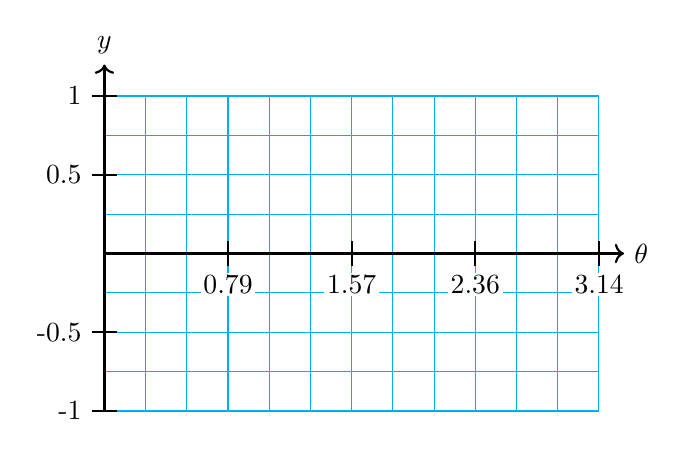
\begin{tikzpicture} [scale=2]
\draw[cyan] (0,-1) grid[xstep=3.14/12, ystep=1/4] (3.14,1);
\draw[black,thick, ->] (0,0) --(3.3,0) node[right] {$\theta$};
\draw[black,thick,->] (0,-1)--(0,1.2) node[above]{$y$};
\foreach \y in {-1,-0.5, 0.5, 1} \draw[black,thick] (.08,\y)--++(-.16,0) node[left]{\y};

\draw[black,thick] (3.14/4,.08)--++(0,-.16) node[below, yshift=-2, fill=white, inner sep=1] {0.79};
\draw[black,thick] (3.14/2,.08)--++(0,-.16) node[below, yshift=-2, fill=white, inner sep=1] {1.57};
\draw[black,thick] (3*3.14/4,.08)--++(0,-.16) node[below, yshift=-2, fill=white, inner sep=1] {2.36};
\draw[black,thick] (pi,.08)--++(0,-.16) node[below, yshift=-2, fill=white, inner sep=1] {3.14};

\end{tikzpicture}
\newline



hp6-3-3ansa sine

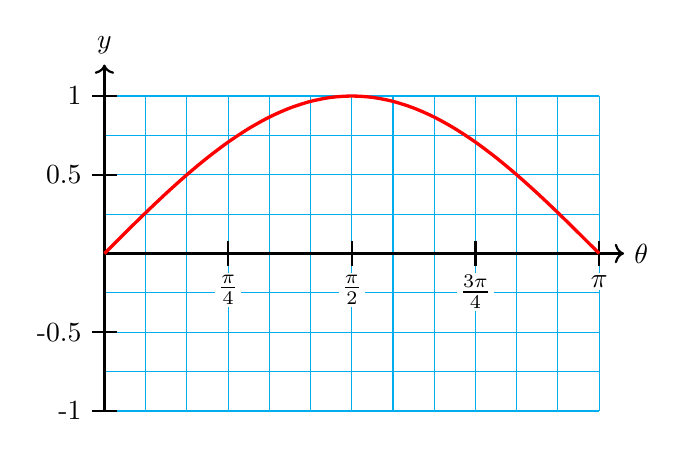
\begin{tikzpicture} [scale=2]
\draw[cyan] (0,-1) grid[xstep=pi/12, ystep=1/4] (pi,1);
\draw[black,thick, ->] (0,0) --(3.3,0) node[right] {$\theta$};
\draw[black,thick,->] (0,-1)--(0,1.2) node[above]{$y$};
\foreach \y in {-1,-0.5, 0.5, 1} \draw[black,thick] (.08,\y)--++(-.16,0) node[left]{\y};

\draw[black,thick] (pi/4,.08)--++(0,-.16) node[below, yshift=-2, fill=white, inner sep=1] {$\frac{\pi}{4}$};
\draw[black,thick] (pi/2,.08)--++(0,-.16) node[below, yshift=-2, fill=white, inner sep=1] {$\frac{\pi}{2}$};
\draw[black,thick] (3*pi/4,.08)--++(0,-.16) node[below, yshift=-2, fill=white, inner sep=1] {$\frac{3\pi}{4}$};
\draw[black,thick] (pi,.08)--++(0,-.16) node[below, yshift=-2, fill=white, inner sep=1] {$\pi$};

\draw[domain=0:pi,smooth,variable=\x,red,very thick] plot ({\x},{sin(deg(\x))});

\end{tikzpicture}
\newline


hp6-3-3ansb

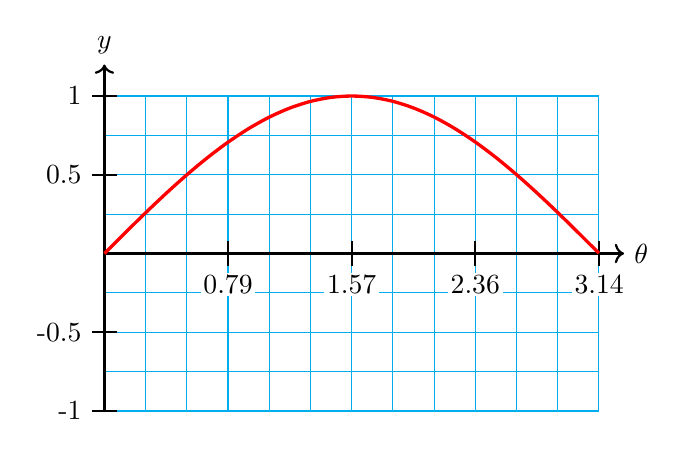
\begin{tikzpicture} [scale=2]
\draw[cyan] (0,-1) grid[xstep=3.14/12, ystep=1/4] (3.14,1);
\draw[black,thick, ->] (0,0) --(3.3,0) node[right] {$\theta$};
\draw[black,thick,->] (0,-1)--(0,1.2) node[above]{$y$};
\foreach \y in {-1,-0.5, 0.5, 1} \draw[black,thick] (.08,\y)--++(-.16,0) node[left]{\y};

\draw[black,thick] (3.14/4,.08)--++(0,-.16) node[below, yshift=-2, fill=white, inner sep=1] {0.79};
\draw[black,thick] (3.14/2,.08)--++(0,-.16) node[below, yshift=-2, fill=white, inner sep=1] {1.57};
\draw[black,thick] (3*3.14/4,.08)--++(0,-.16) node[below, yshift=-2, fill=white, inner sep=1] {2.36};
\draw[black,thick] (pi,.08)--++(0,-.16) node[below, yshift=-2, fill=white, inner sep=1] {3.14};

\draw[domain=0:3.14,smooth,variable=\x,red,very thick] plot ({\x},{sin(deg(\x))});

\end{tikzpicture}
\newline



hp6-3-5 grid
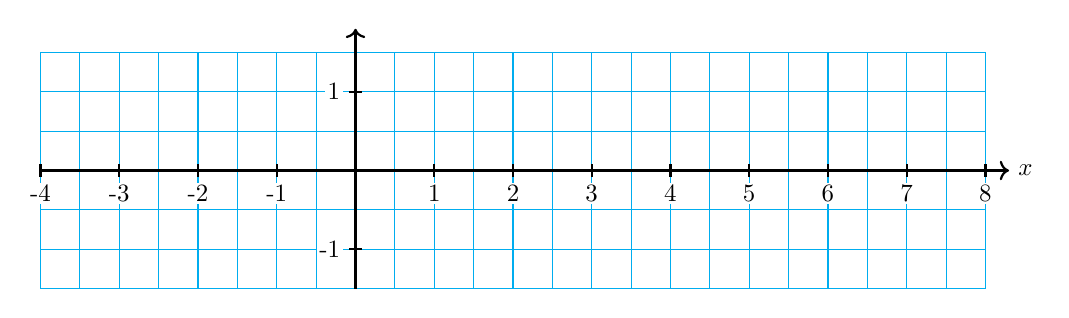
\begin{tikzpicture}

\draw[cyan] (-4,-1.5) grid[step=1/2] (8,1.5);
\draw[black,thick,->] (-4,0)--(8.3,0) node[right, scale=.9]{$x$};
\draw[black,thick,->] (0,-1.5)--(0,1.8) ;

\foreach \x in {-4, -3,-2,-1, 1, 2, ..., 8} \draw[black,thick] (\x,0.08) -- ++(0,-.16) node[below, yshift=-2, fill=white, inner sep = 1, scale=.9] {\x};

\foreach \y in {-1, 1} \draw[black,thick] (0.08, \y) -- ++(-.16,0) node[left, xshift=-2, fill=white, inner sep = 1, scale=.9] {\y};

\end{tikzpicture}
\newline



hp6-3-5ans sine
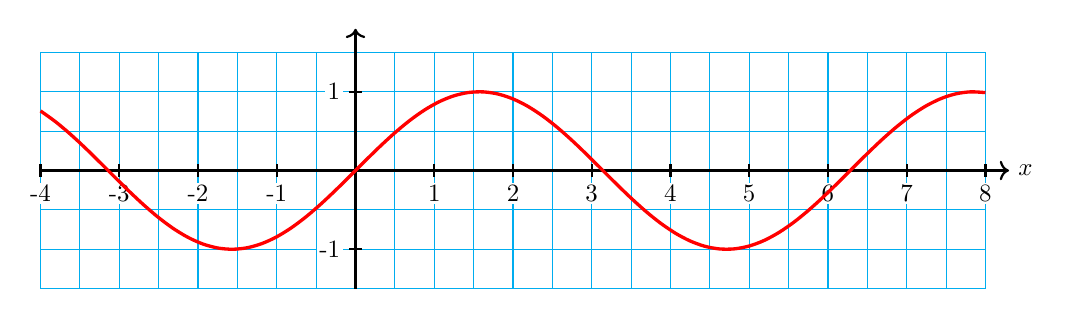
\begin{tikzpicture}

\draw[cyan] (-4,-1.5) grid[step=1/2] (8,1.5);
\draw[black,thick,->] (-4,0)--(8.3,0) node[right, scale=.9]{$x$};
\draw[black,thick,->] (0,-1.5)--(0,1.8) ;

\foreach \x in {-4, -3,-2,-1, 1, 2, ..., 8} \draw[black,thick] (\x,0.08) -- ++(0,-.16) node[below, yshift=-2, fill=white, inner sep = 1, scale=.9] {\x};

\foreach \y in {-1, 1} \draw[black,thick] (0.08, \y) -- ++(-.16,0) node[left, xshift=-2, fill=white, inner sep = 1, scale=.9] {\y};

\draw[samples=65,domain=-4:8,smooth,variable=\x,red,very thick] plot ({\x},{sin(deg(\x))});

\end{tikzpicture}
\newline



hp6-3-7 grid
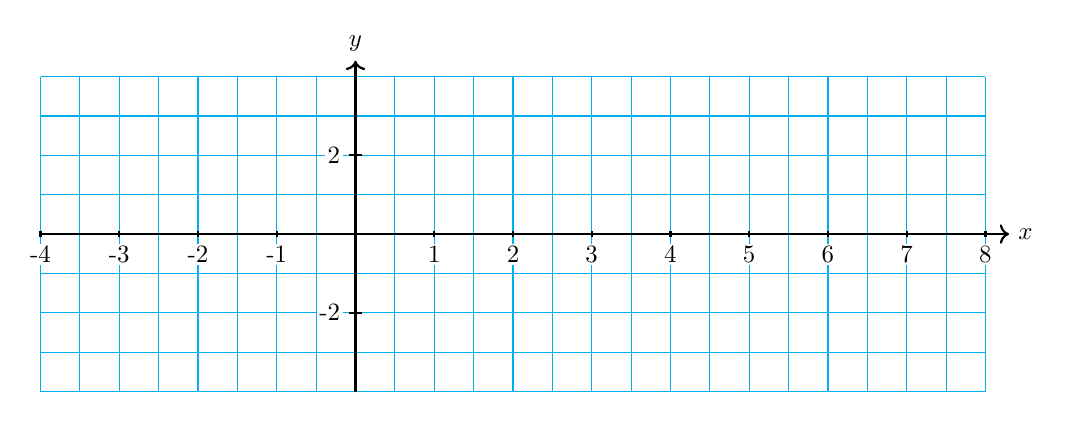
\begin{tikzpicture} [yscale=1/2]

\draw[cyan] (-4,-4) grid[xstep=1/2] (8,4);
\draw[black,thick,->] (-4,0)--(8.3,0) node[right, scale=.9]{$x$};
\draw[black,thick,->] (0,-4)--(0,4.4) node[above, scale=.9]{$y$};

\foreach \x in {-4, -3,-2,-1, 1, 2, ..., 8} \draw[black,thick] (\x,0.08) -- ++(0,-.16) node[below, yshift=-2, fill=white, inner sep = 1, scale=.9] {\x};

\foreach \y in {-2, 2} \draw[black,thick] (0.08, \y) -- ++(-.16,0) node[left, xshift=-2, fill=white, inner sep = 1, scale=.9] {\y};

\end{tikzpicture}
\newline



hp6-3-7ans tangent
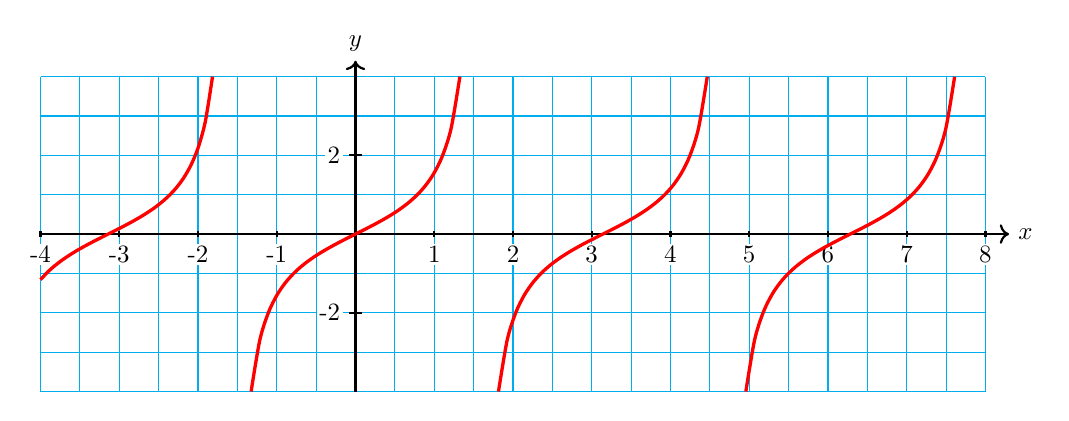
\begin{tikzpicture} [yscale=1/2]

\draw[cyan] (-4,-4) grid[xstep=1/2] (8,4);
\draw[black,thick,->] (-4,0)--(8.3,0) node[right, scale=.9]{$x$};
\draw[black,thick,->] (0,-4)--(0,4.4) node[above, scale=.9]{$y$};

\foreach \x in {-4, -3,-2,-1, 1, 2, ..., 8} \draw[black,thick] (\x,0.08) -- ++(0,-.16) node[below, yshift=-2, fill=white, inner sep = 1, scale=.9] {\x};

\foreach \y in {-2, 2} \draw[black,thick] (0.08, \y) -- ++(-.16,0) node[left, xshift=-2, fill=white, inner sep = 1, scale=.9] {\y};

\draw[domain={-4:atan(4)*pi/180-pi}, smooth, variable=\x,red,very thick] plot ({\x},{tan(deg(\x))}) ;
\draw[domain={-atan(4)*pi/180:atan(4)*pi/180}, smooth, variable=\x,red,very thick] plot ({\x},{tan(deg(\x))}) ;
\draw[domain={pi-atan(4)*pi/180:pi+atan(4)*pi/180}, smooth, variable=\x,red,very thick] plot ({\x},{tan(deg(\x))}) ;
\draw[domain={2*pi-atan(4)*pi/180:2*pi+atan(4)*pi/180}, smooth, variable=\x,red,very thick] plot ({\x},{tan(deg(\x))}) ;

\end{tikzpicture}
\newline



hp6-3-8 grid
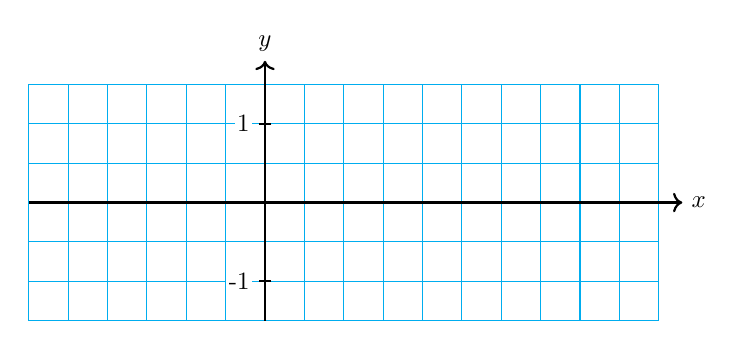
\begin{tikzpicture} 

\draw[cyan] (-3,-3/2) grid[step=1/2] (5,3/2);
\draw[black,thick,->] (-3,0)--(5.3,0) node[right, scale=.9]{$x$};
\draw[black,thick,->] (0,-3/2)--(0,1.8) node[above, scale=.9]{$y$};

\foreach \y in {-1, 1} \draw[black,thick] (0.08, \y) -- ++(-.16,0) node[left, xshift=-2, fill=white, inner sep = 1, scale=.9] {\y};

\end{tikzpicture}
\newline



hp6-3-8 grid
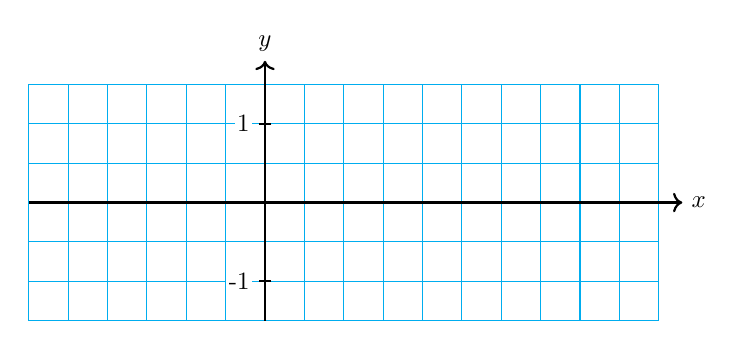
\begin{tikzpicture} 

\draw[cyan] (-3,-3/2) grid[step=1/2] (5,3/2);
\draw[black,thick,->] (-3,0)--(5.3,0) node[right, scale=.9]{$x$};
\draw[black,thick,->] (0,-3/2)--(0,1.8) node[above, scale=.9]{$y$};

\foreach \y in {-1, 1} \draw[black,thick] (0.08, \y) -- ++(-.16,0) node[left, xshift=-2, fill=white, inner sep = 1, scale=.9] {\y};

\end{tikzpicture}
\newline



hp6-3-9 sine 

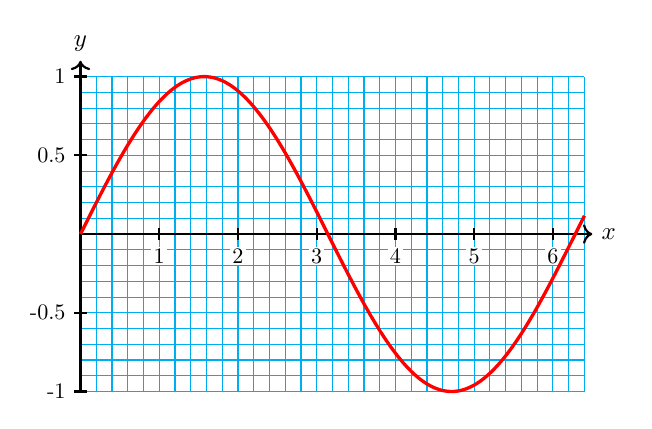
\begin{tikzpicture} [yscale=2]

\draw[cyan] (0,-1) grid[xstep=1/5, ystep=1/10] (6.4,1);
\draw[black,thick,->] (0,0)--(6.5,0) node[right, scale=.9]{$x$};
\draw[black,thick,->] (0,-1)--(0,1.1) node[above, scale=.9]{$y$};

\foreach \x in { 1, 2, ..., 6} \draw[black,thick] (\x,0.04) -- ++(0,-.08) node[below, yshift=-2, fill=white, inner sep = 1, scale=.8] {\x};

\foreach \y in {-1, -0.5, 0.5, 1} \draw[black,thick] (0.08, \y) -- ++(-.16,0) node[left, xshift=-2, fill=white, inner sep = 1, scale=.8] {\y};

\draw[samples=65,domain=-0:6.4,smooth,variable=\x,red,very thick] plot ({\x},{sin(deg(\x))});

\end{tikzpicture}
\newline



hp6-3-10 unit circle on grid

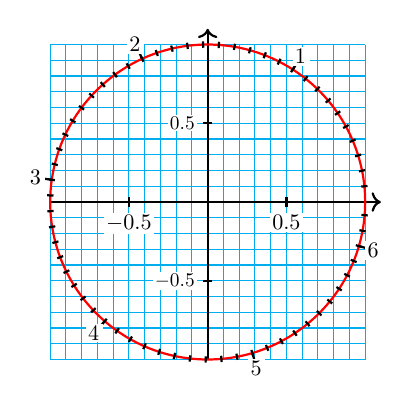
\begin{tikzpicture} [scale=2]

\draw[cyan] (-1.0001,-1.0001) grid[step = 0.1] (1,1);
\draw[black, thick, ->] (-1,0)--(1.1,0);
\draw[black, thick, ->] (0,-1)--(0,1.1);

\draw[red,thick] (0,0) circle (1cm);

\foreach \i in {0.1, 0.2, ..., 6.2} {
 \draw[black, thick] ({deg(\i)}:.98) -- ({deg(\i)}:1.02);
};
\foreach \i in {1,2, ..., 6} {
 \draw[black, thick] ({deg(\i)}:1) -- ({deg(\i)}:1.05);
 \node[text width=.2cm, fill=white, inner sep=1, scale=.8] at ({deg(\i)}:1.1) { $\i$};
};
\foreach \i in {-0.5, 0.5} {
 \draw[black, thick] (0.03,\i) -- (-0.03,\i) node[left, xshift=-2, fill=white, inner sep=1, scale=.7]{ $\i$};
 \draw[black, thick] (\i,0.03) -- (\i,-0.03) node[below, yshift=-2, fill=white, inner sep=1, scale=.8]{$\i$};
};

\end{tikzpicture}
\newline



hp6-3-11 cosine 

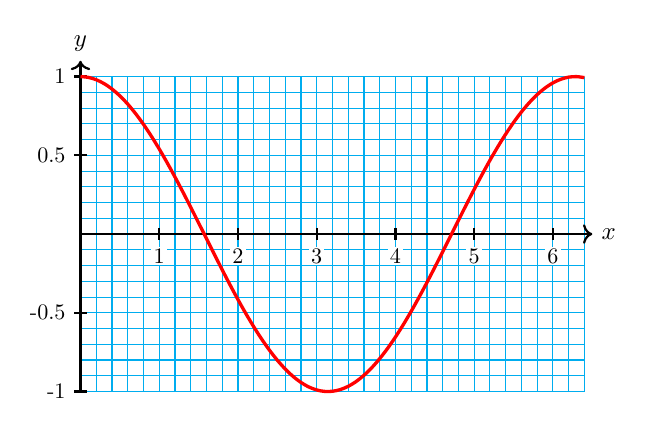
\begin{tikzpicture} [yscale=2]

\draw[cyan] (0,-1) grid[xstep=1/5, ystep=1/10] (6.4,1);
\draw[black,thick,->] (0,0)--(6.5,0) node[right, scale=.9]{$x$};
\draw[black,thick,->] (0,-1)--(0,1.1) node[above, scale=.9]{$y$};

\foreach \x in { 1, 2, ..., 6} \draw[black,thick] (\x,0.04) -- ++(0,-.08) node[below, yshift=-2, fill=white, inner sep = 1, scale=.8] {\x};

\foreach \y in {-1, -0.5, 0.5, 1} \draw[black,thick] (0.08, \y) -- ++(-.16,0) node[left, xshift=-2, fill=white, inner sep = 1, scale=.8] {\y};

\draw[samples=65,domain=-0:6.4,smooth,variable=\x,red,very thick] plot ({\x},{cos(deg(\x))});

\end{tikzpicture}
\newline



hp6-3-13 tan 

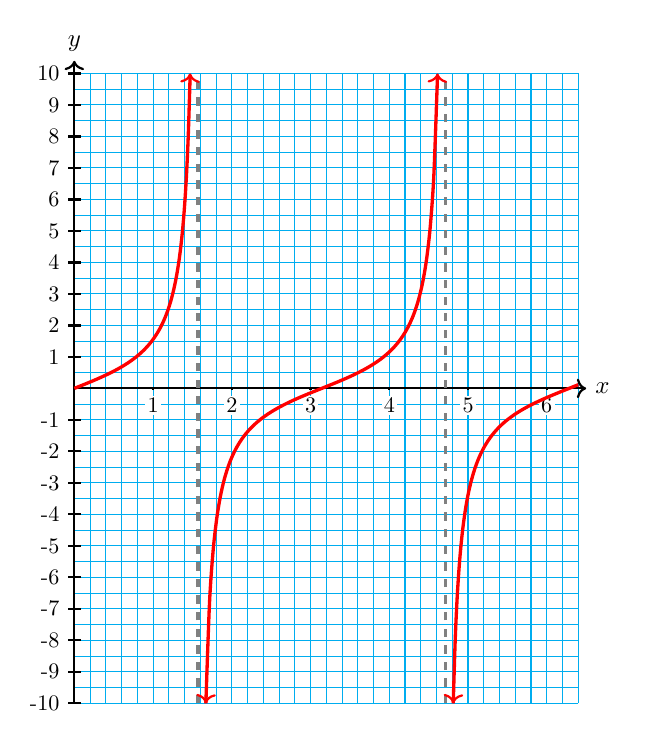
\begin{tikzpicture} [yscale=.4]

\draw[cyan] (0,-10) grid[xstep=1/5, ystep=1/2] (6.4,10);
\draw[black,thick,->] (0,0)--(6.5,0) node[right, scale=.9]{$x$};
\draw[black,thick,->] (0,-10)--(0,10.4) node[above, scale=.9]{$y$};
\draw[gray, very thick,dashed] (pi/2,-10)--++(0,20);
\draw[gray, very thick,dashed] (3*pi/2,-10)--++(0,20);

\foreach \x in { 1,2,..., 6} \draw[black,thick] (\x,0.04) -- ++(0,-.08) node[below, yshift=-2, fill=white, inner sep = 1, scale=.8] {\x};

\foreach \y in {-10, -9,...,-1, 1,2,..., 10} \draw[black,thick] (0.08, \y) -- ++(-.16,0) node[left, xshift=-2, fill=white, inner sep = 1, scale=.8] {\y};

\draw[samples=65,domain=0:{atan(10)*pi/180},smooth,variable=\x,red,very thick] plot ({\x},{tan(deg(\x))});
\draw[red,thick,->] ($ atan(9.5)*pi/180*(1,0)+(0,9.5)$)--($ atan(10)*pi/180*(1,0)+(0,10)$);

\draw[samples=65,domain={pi-atan(10)*pi/180}:{pi+atan(10)*pi/180},smooth,variable=\x,red,very thick] plot ({\x},{tan(deg(\x))});
\draw[red,thick,->] ($ atan(9.5)*pi/180*(1,0)+(pi,9.5)$)--($ atan(10)*pi/180*(1,0)+(pi,10)$);
\draw[red,thick,->] ($ atan(9.5)*pi/180*(-1,0)+(pi,-9.5)$)--($ atan(10)*pi/180*(-1,0)+(pi,-10)$);

\draw[samples=65,domain={2*pi-atan(10)*pi/180}:6.4,smooth,variable=\x,red,very thick] plot ({\x},{tan(deg(\x))});
\draw[red,thick,->] ($ atan(9.5)*pi/180*(-1,0)+(2*pi,-9.5)$)--($ atan(10)*pi/180*(-1,0)+(2*pi,-10)$);

\end{tikzpicture}
\newline


hp6-3-59 grid
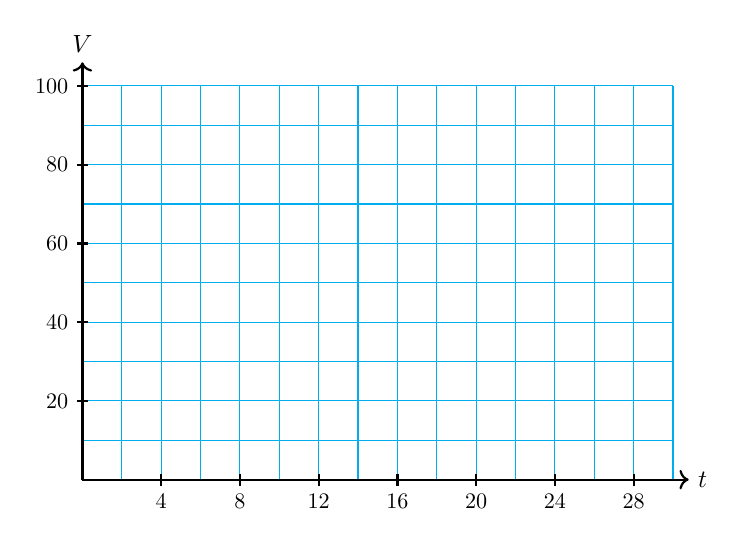
\begin{tikzpicture} [xscale=.25, yscale=.05]

\draw[cyan] (0,0) grid[xstep=2,ystep=10] (30,100);
\draw[black,thick,->] (0,0)--(30.8,0) node[right, scale=.9]{$t$};
\draw[black,thick,->] (0,0)--(0, 106) node[above, scale=.9]{$V$};
\foreach \x in {4, 8, ..., 28} \draw[black, thick] (\x,1.5)--++(0,-3) node[below, scale=0.8]{\x};

\foreach \y in {20,40, ..., 100} \draw[black, thick] (.3,\y)--++(-.6,0) node[left, scale=0.8]{\y};
\end{tikzpicture}
\newline


hp6-3-59ans sinusoidal graph
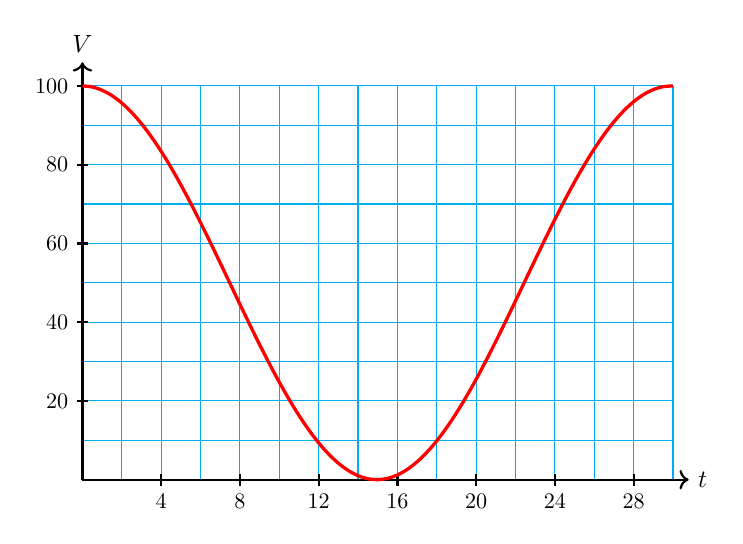
\begin{tikzpicture} [xscale=.25, yscale=.05]

\draw[cyan] (0,0) grid[xstep=2,ystep=10] (30,100);
\draw[black,thick,->] (0,0)--(30.8,0) node[right, scale=.9]{$t$};
\draw[black,thick,->] (0,0)--(0, 106) node[above, scale=.9]{$V$};
\foreach \x in {4, 8, ..., 28} \draw[black, thick] (\x,1.5)--++(0,-3) node[below, scale=0.8]{\x};

\foreach \y in {20,40, ..., 100} \draw[black, thick] (.3,\y)--++(-.6,0) node[left, scale=0.8]{\y};
\draw[samples=65,domain=-0:30,smooth,variable=\x,red,very thick] plot ({\x},{50+50*cos(deg(0.21*\x))});
\end{tikzpicture}
\newline


hp6-3-60 grid
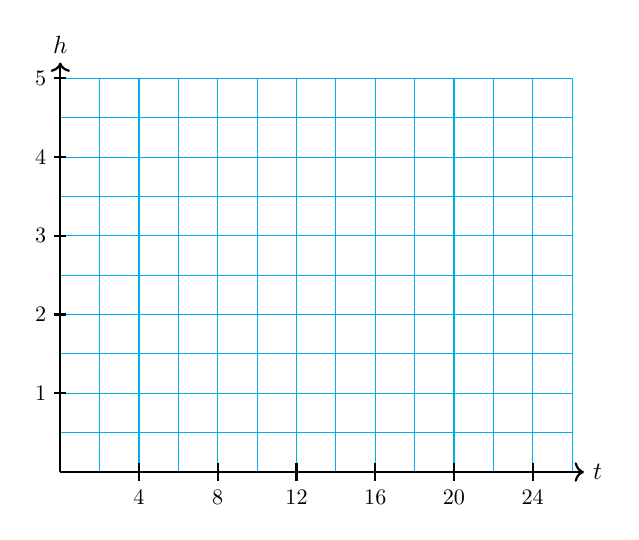
\begin{tikzpicture} [xscale=.25, yscale=1]

\draw[cyan] (0,0) grid[xstep=2,ystep=1/2] (26,5);
\draw[black,thick,->] (0,0)--(26.6,0) node[right, scale=.9]{$t$};
\draw[black,thick,->] (0,0)--(0, 5.2) node[above, scale=.9]{$h$};
\foreach \x in {4, 8, ..., 24} \draw[black, thick] (\x,.12)--++(0,-.24) node[below, scale=0.8]{\x};

\foreach \y in {1,2,...,5} \draw[black, thick] (.3,\y)--++(-.6,0) node[left, scale=0.8]{\y};
\end{tikzpicture}
\newline


hp6-3-61 grid
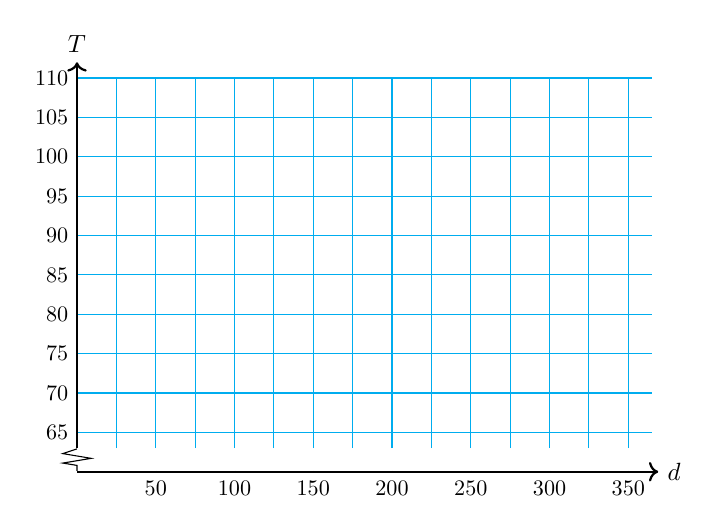
\begin{tikzpicture} [xscale=.02, yscale=.1]

\draw[cyan] (0,63) grid[xstep=25,ystep=5] (365,110);
\draw[black,thick,->] (0,60)--++(369,0) node[right, scale=.9]{$d$};
\draw[black,thick,->] (0,63)--(0, 112) node[above, scale=.9]{$T$};
\foreach \x in {50, 100, ..., 350} \draw[black, thick] (\x,60.12)--++(0,-.24) node[below, scale=0.8]{\x};
\coordinate (O) at (0,62);
\draw[black] (O)++(0,.9)--++(-9, -.6)--++(18,-.6)--++(-18,-.6)--++(9,-.3) -- ++(0, -.7);

\foreach \y in {65, 70, ...,110} \draw[black, thick] (.3,\y)--++(-.6,0) node[left, scale=0.8]{\y};
\end{tikzpicture}
\newline


hp6-3-61ans sinusoidal graph
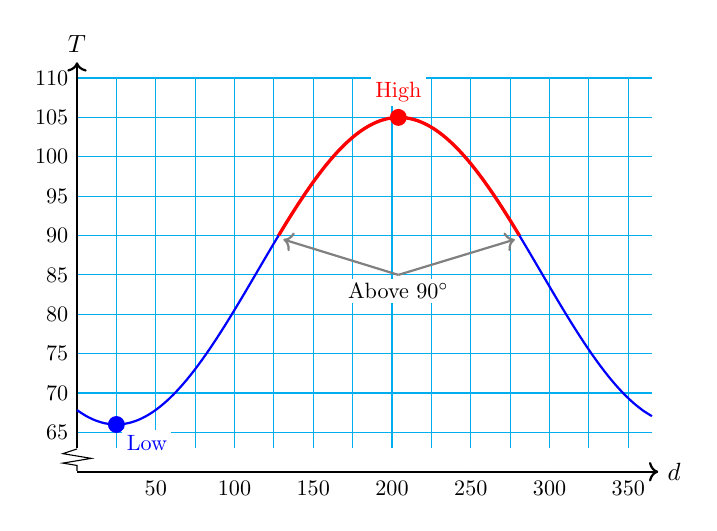
\begin{tikzpicture} [xscale=.02, yscale=.1]

\draw[cyan] (0,63) grid[xstep=25,ystep=5] (365,110);
\draw[black,thick,->] (0,60)--++(369,0) node[right, scale=.9]{$d$};
\draw[black,thick,->] (0,63)--(0, 112) node[above, scale=.9]{$T$};
\foreach \x in {50, 100, ..., 350} \draw[black, thick] (\x,60.12)--++(0,-.24) node[below, scale=0.8]{\x};
\draw[black] (0,62.9)--++(-9, -.6)--++(18,-.6)--++(-18,-.6)--++(9,-.3) -- ++(0, -.7);

\foreach \y in {65, 70, ...,110} \draw[black, thick] (.3,\y)--++(-.6,0) node[left, scale=0.8]{\y};
\draw[samples=65,domain=0:365,smooth,variable=\x,blue, thick] plot ({\x},{85.5-19.5*cos(deg(0.0175*\x - 0.436))});
\draw[samples=65,domain=128:280.89,smooth,variable=\x,red,very thick] plot ({\x},{85.5-19.5*cos(deg(0.0175*\x - 0.436))});

\filldraw[red] (204, 105) ellipse (5cm and 1cm) node[above, fill=white, inner sep = 2, yshift = 4, scale = .8] {High};
\filldraw[blue] (25, 66) ellipse (5cm and 1cm) node[below right, fill=white, inner sep = 2, xshift=2, yshift = -2, scale = .8] {Low};
\draw[gray,thick,<-] (131, 89.5)--(204,85);
\draw[gray,thick,<-] (278, 89.5)--(204,85);
\node[fill=white, inner sep = 2, scale=.8] at (204,83) {Above $90\degree$};
\end{tikzpicture}
\newline


hp6-3-62 grid
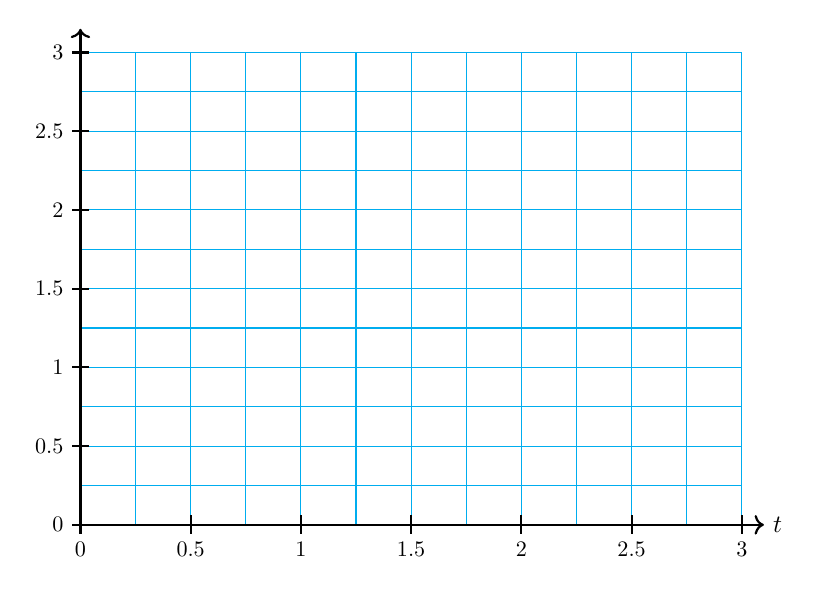
\begin{tikzpicture} [xscale=2.8, yscale=2]
\draw[cyan] (0,0) grid[step=.25] (3,3);
\draw[black,thick,->] (0,0)--++(3.1,0) node[right, scale=.9]{$t$};
\draw[black,thick,->] (0,0)--(0, 3.15);
\foreach \x in {0,0.5,1,1.5,2,2.5,3} \draw[black, thick] (\x,0.06)--++(0,-.12) node[below, scale=0.8]{\x};

\foreach \y in {0,0.5,1,1.5,2,2.5,3} \draw[black, thick] (.04,\y)--++(-.08,0) node[left, scale=0.8]{\y};
\end{tikzpicture}
\newline


hp6-3-63 unit circle
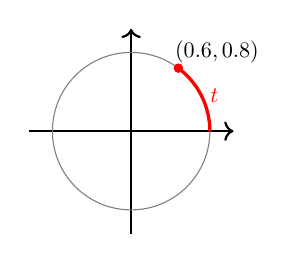
\begin{tikzpicture}
\draw[black,thick,->] (-1.3,0)--(1.3,0);
\draw[black,thick,->] (0,-1.3)--(0,1.3);
\draw[gray] (0,0) circle (1cm);
\draw[red, very thick] (1,0) arc (0:{atan(4/3)}:1) node[right, midway, scale=0.8] {$t$};
\filldraw[red] (0.6,0.8) circle (1.5pt) node[anchor=south west, xshift=-4, yshift=-1, scale=0.8, text=black] {$(0.6,0.8)$};

\end{tikzpicture}
\newline


hp6-3-64 unit circle
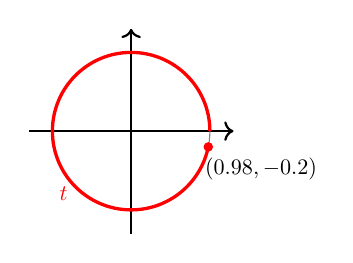
\begin{tikzpicture}
\draw[black,thick,->] (-1.3,0)--(1.3,0);
\draw[black,thick,->] (0,-1.3)--(0,1.3);
\draw[gray] (0,0) circle (1cm);
\draw[red, very thick] (1,0) arc (0:{360-atan(10/49)}:1) node[ left, midway, xshift=.3cm, yshift=-.9cm,  scale=0.8] {$t$};
\filldraw[red] (0.98,-0.2) circle (1.5pt) node[anchor=north west, xshift=-4, yshift=-1, scale=0.8, text=black] {$(0.98,-0.2)$};

\end{tikzpicture}
\newline


hp6-3-65 unit circle
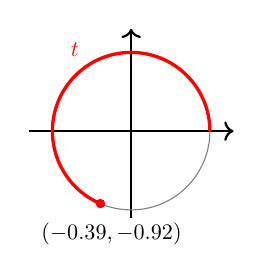
\begin{tikzpicture}
\draw[black,thick,->] (-1.3,0)--(1.3,0);
\draw[black,thick,->] (0,-1.1)--(0,1.3);
\draw[gray] (0,0) circle (1cm);
\draw[red, very thick] (1,0) arc (0:{180+atan(92/39)}:1) node[above left, midway, scale=0.8] {$t$};
\filldraw[red] (-0.39,-0.92) circle (1.5pt) node[anchor=north , xshift=4, yshift=-4, scale=0.8, text=black] {$(-0.39,-0.92)$};

\end{tikzpicture}
\newline


hp6-3-66 unit circle
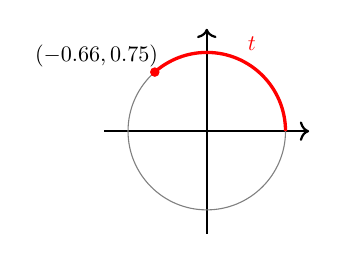
\begin{tikzpicture}
\draw[black,thick,->] (-1.3,0)--(1.3,0);
\draw[black,thick,->] (0,-1.3)--(0,1.3);
\draw[gray] (0,0) circle (1cm);
\draw[red, very thick] (1,0) arc (0:{180-atan(75/66)}:1) node[ above right, midway,scale=0.8] {$t$};
\filldraw[red] (-0.66,0.75) circle (1.5pt) node[anchor=south east, xshift=4, yshift=-1, scale=0.8, text=black] {$(-0.66,0.75)$};

\end{tikzpicture}
\newline





hp6-3-67ans labeled trig graphs


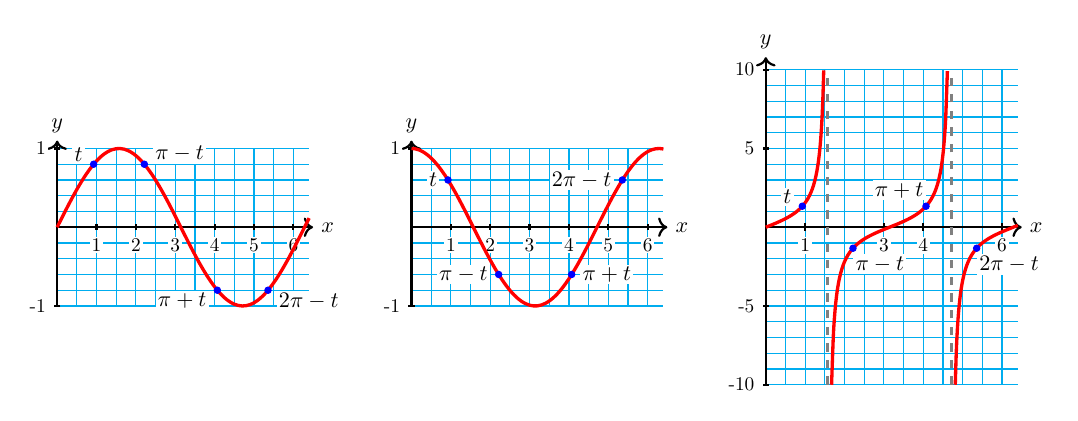
\begin{tikzpicture} [xscale=1/2]

\draw[cyan] (0,-1) grid[xstep=1/2, ystep=1/5] (6.4,1);
\draw[black,thick,->] (0,0)--(6.5,0) node[right, scale=.8]{$x$};
\draw[black,thick,->] (0,-1)--(0,1.1) node[above, scale=.8]{$y$};

\foreach \x in { 1, 2, ..., 6} \draw[black,thick] (\x,0.04) -- ++(0,-.08) node[below, yshift=-2, fill=white, inner sep = 1, scale=.7] {\x};
\foreach \y in {-1, 1} \draw[black,thick] (0.08, \y) -- ++(-.16,0) node[left, xshift=-2, fill=white, inner sep = 1, scale=.7] {\y};

\draw[samples=65,domain=-0:6.4,smooth,variable=\x,red,very thick] plot ({\x},{sin(deg(\x))});

\coordinate (A) at ($ asin(0.8)*pi/180*(1,0)+(0,0.8)$);
\filldraw[blue] (A) ellipse (.08cm and .04cm) node[anchor=south east, xshift=-3, fill=white, inner sep=1, scale=.8,text=black]{$t$};
\coordinate (B) at ($ asin(0.8))*pi/180*(-1,0)+(pi,0.8)$);
\filldraw[blue] (B) ellipse (.08cm and .04cm) node[anchor=south west, xshift=3, fill=white, inner sep=1, scale=.8,text=black]{$\pi-t$};
\coordinate (C) at ($ asin(0.8))*pi/180*(1,0)+(pi,-0.8)$);
\filldraw[blue] (C) ellipse (.08cm and .04cm) node[anchor=north east, xshift=-3, fill=white, inner sep=1, scale=.8,text=black]{$\pi+t$};
\coordinate (D) at ($ asin(0.8))*pi/180*(-1,0)+(2*pi,-0.8)$);
\filldraw[blue] (D) ellipse (.08cm and .04cm) node[anchor=north west, xshift=3, fill=white, inner sep=1, scale=.8,text=black]{$2\pi-t$};


%second graph: cosine
\draw[cyan] (9,-1) grid[xstep=1/2, ystep=1/5] (15.4,1);
\draw[black,thick,->] (9,0)--++(6.5,0) node[right, scale=.8]{$x$};
\draw[black,thick,->] (9,-1)--++(0,2.1) node[above, scale=.8]{$y$};

\foreach \x [evaluate=\x as \xi using int(\x+9)] in { 1, 2, ..., 6} \draw[black,thick] (\xi,0.04) -- ++(0,-.08) node[below, yshift=-2, fill=white, inner sep = 1, scale=.7] {\x};
\foreach \y in {-1, 1} \draw[black,thick] (9.08, \y) -- ++(-.16,0) node[left, xshift=-2, fill=white, inner sep = 1, scale=.7] {\y};

\draw[samples=65,domain=-0:6.4,smooth,variable=\x,red,very thick] plot ({\x+9},{cos(deg(\x))});

\coordinate (A) at ($ asin(0.8)*pi/180*(1,0)+(9,0.6)$);
\filldraw[blue] (A) ellipse (.08cm and .04cm) node[anchor= east, xshift=-3, fill=white, inner sep=1, scale=.8,text=black]{$t$};
\coordinate (B) at ($ asin(0.8)*pi/180*(-1,0)+(pi+9,-0.6)$);
\filldraw[blue] (B) ellipse (.08cm and .04cm) node[anchor= east, xshift=-3, fill=white, inner sep=1, scale=.8,text=black]{$\pi-t$};
\coordinate (C) at ($ asin(0.8))*pi/180*(1,0)+(9+pi,-0.6)$);
\filldraw[blue] (C) ellipse (.08cm and .04cm) node[anchor=west, xshift=3, fill=white, inner sep=1, scale=.8,text=black]{$\pi+t$};
\coordinate (D) at ($ asin(0.8))*pi/180*(-1,0)+(9+2*pi,0.6)$);
\filldraw[blue] (D) ellipse (.08cm and .04cm) node[anchor=east, xshift=-3, fill=white, inner sep=1, scale=.8,text=black]{$2\pi-t$};

%third graph: tangent
\draw[cyan] (18,-2) grid[xstep=1/2, ystep=.2] (24.4,2);
\draw[black,thick,->] (18,0)--(24.5,0) node[right, scale=.8]{$x$};
\draw[black,thick,->] (18,-2)--(18,2.16) node[above, scale=.8]{$y$};
\draw[gray, very thick,dashed] (18,0)++(pi/2,-2)--++(0,4);
\draw[gray, very thick,dashed] (18,0)++(3*pi/2,-2)--++(0,4);
\foreach \x [evaluate=\x as \xi using int(\x+18)] in { 1,3,4, 6} \draw[black,thick] (\xi,0.05) -- ++(0,-.1) node[below, yshift=-2, fill=white, inner sep = 1, scale=.7] {\x};
\foreach \y [evaluate=\y as \yi using (\y *.2)]  in {-10, -5, 5, 10} \draw[black,thick] (18.08, \yi) -- ++(-.16,0) node[left, xshift=-2, fill=white, inner sep = 1, scale=.7] {\y};

\draw[samples=65,domain=0:{atan(10)*pi/180},smooth,variable=\x,red,very thick] plot ({\x+18},{0.2*tan(deg(\x))});
\draw[samples=65,domain={pi-atan(10)*pi/180}:{pi+atan(10)*pi/180},smooth,variable=\x,red,very thick] plot ({\x+18},{0.2*tan(deg(\x))});
\draw[samples=65,domain={2*pi-atan(10)*pi/180}:6.4,smooth,variable=\x,red,very thick] plot ({\x+18},{0.2*tan(deg(\x))});

\coordinate (A) at ($ asin(0.8)*pi/180*(1,0)+(18,4/15)$);
\filldraw[blue] (A) ellipse (.08cm and .04cm) node[anchor=south east, xshift=-3, fill=white, inner sep=1, scale=.8,text=black]{$t$};
\coordinate (B) at ($ asin(0.8)*pi/180*(-1,0)+(pi+18,-4/15)$);
\filldraw[blue] (B) ellipse (.08cm and .04cm) node[anchor=north west, yshift=-2, fill=white, inner sep=1, scale=.8,text=black]{$\pi-t$};
\coordinate (C) at ($ asin(0.8))*pi/180*(1,0)+(18+pi,4/15)$);
\filldraw[blue] (C) ellipse (.08cm and .04cm) node[anchor=south east, yshift=2, fill=white, inner sep=1, scale=.8,text=black]{$\pi+t$};
\coordinate (D) at ($ asin(0.8))*pi/180*(-1,0)+(18+2*pi,-4/15)$);
\filldraw[blue] (D) ellipse (.08cm and .04cm) node[anchor=north west, yshift=-2, fill=white, inner sep=1, scale=.8,text=black]{$2\pi-t$};


\end{tikzpicture}
\newline






hp6-3-69ans labeled trig graphs


\begin{tikzpicture} [xscale=1/2]

\draw[cyan] (0,-1) grid[xstep=1/2, ystep=1/5] (6.4,1);
\draw[black,thick,->] (0,0)--(6.5,0) node[right, scale=.8]{$x$};
\draw[black,thick,->] (0,-1)--(0,1.1) node[above, scale=.8]{$y$};

\foreach \x in { 1, 2, ..., 6} \draw[black,thick] (\x,0.04) -- ++(0,-.08) node[below, yshift=-2, fill=white, inner sep = 1, scale=.7] {\x};
\foreach \y in {-1, 1} \draw[black,thick] (0.08, \y) -- ++(-.16,0) node[left, xshift=-2, fill=white, inner sep = 1, scale=.7] {\y};

\draw[samples=65,domain=-0:6.4,smooth,variable=\x,red,very thick] plot ({\x},{sin(deg(\x))});

\coordinate (A) at ($ asin(0.92)*pi/180*(1,0)+(pi,-0.92)$);
\filldraw[blue] (A) ellipse (.08cm and .04cm) node[anchor=south west, yshift=2, fill=white, inner sep=1, scale=.8,text=black]{$t$};

\coordinate (D) at ($ asin(0.92))*pi/180*(-1,0)+(pi,0.92)$);
\filldraw[blue] (D) ellipse (.08cm and .04cm) node[anchor=south west, xshift=2, fill=white, inner sep=1, scale=.8,text=black]{$2\pi-t$};


%second graph: cosine
\draw[cyan] (9,-1) grid[xstep=1/2, ystep=1/5] (15.4,1);
\draw[black,thick,->] (9,0)--++(6.5,0) node[right, scale=.8]{$x$};
\draw[black,thick,->] (9,-1)--++(0,2.1) node[above, scale=.8]{$y$};

\foreach \x [evaluate=\x as \xi using int(\x+9)] in { 1, 2, ..., 6} \draw[black,thick] (\xi,0.04) -- ++(0,-.08) node[below, yshift=-2, fill=white, inner sep = 1, scale=.7] {\x};
\foreach \y in {-1, 1} \draw[black,thick] (9.08, \y) -- ++(-.16,0) node[left, xshift=-2, fill=white, inner sep = 1, scale=.7] {\y};

\draw[samples=65,domain=-0:6.4,smooth,variable=\x,red,very thick] plot ({\x+9},{cos(deg(\x))});

\coordinate (A) at ($ asin(0.92)*pi/180*(1,0)+(9+pi,-0.39)$);
\filldraw[blue] (A) ellipse (.08cm and .04cm) node[anchor=north west, xshift=2, fill=white, inner sep=1, scale=.8,text=black]{$t$};

\coordinate (D) at ($ asin(0.92))*pi/180*(-1,0)+(9+pi,-0.39)$);
\filldraw[blue] (D) ellipse (.08cm and .04cm) node[anchor=north east, xshift=-3, fill=white, inner sep=1, scale=.8,text=black]{$2\pi-t$};

%third graph: tangent
\draw[cyan] (18,-2) grid[xstep=1/2, ystep=.2] (24.4,2);
\draw[black,thick,->] (18,0)--(24.5,0) node[right, scale=.8]{$x$};
\draw[black,thick,->] (18,-2)--(18,2.16) node[above, scale=.8]{$y$};
\draw[gray, very thick,dashed] (18,0)++(pi/2,-2)--++(0,4);
\draw[gray, very thick,dashed] (18,0)++(3*pi/2,-2)--++(0,4);
\foreach \x [evaluate=\x as \xi using int(\x+18)] in { 1,3,4, 6} \draw[black,thick] (\xi,0.05) -- ++(0,-.1) node[below, yshift=-2, fill=white, inner sep = 1, scale=.7] {\x};
\foreach \y [evaluate=\y as \yi using (\y *.2)]  in {-10, -5, 5, 10} \draw[black,thick] (18.08, \yi) -- ++(-.16,0) node[left, xshift=-2, fill=white, inner sep = 1, scale=.7] {\y};

\draw[samples=65,domain=0:{atan(10)*pi/180},smooth,variable=\x,red,very thick] plot ({\x+18},{0.2*tan(deg(\x))});
\draw[samples=65,domain={pi-atan(10)*pi/180}:{pi+atan(10)*pi/180},smooth,variable=\x,red,very thick] plot ({\x+18},{0.2*tan(deg(\x))});
\draw[samples=65,domain={2*pi-atan(10)*pi/180}:6.4,smooth,variable=\x,red,very thick] plot ({\x+18},{0.2*tan(deg(\x))});

\coordinate (A) at ($ asin(0.92)*pi/180*(1,0)+(18+pi,92/39/5)$);
\filldraw[blue] (A) ellipse (.08cm and .04cm) node[anchor=south east, xshift=-2, fill=white, inner sep=1, scale=.8,text=black]{$t$};

\coordinate (D) at ($ asin(0.92))*pi/180*(-1,0)+(18+pi,-92/39/5)$);
\filldraw[blue] (D) ellipse (.08cm and .04cm) node[anchor=north west, xshift=3, fill=white, inner sep=1, scale=.8,text=black]{$2\pi-t$};

\end{tikzpicture}
\newline



hp6-3-71ans
\begin{tikzpicture} [scale=.2]
\draw[cyan] (-10,-10) grid[step=2] (10,10);
\draw[black,thick,->] (-10,0)--(10.8,0) node[right]{$x$};
\draw[black,thick,->] (0,-10)--(0,10.8) node[above]{$y$};
\foreach \i in {-10,10} {
 \draw[black,thick] (\i,0.4)--++(0,-.8) node[below, yshift=-2, fill=white, inner sep=1pt, scale=.9] {\i};
 \draw[black,thick] (0.4,\i)--++(-0.8,0) node[left, xshift=-2, fill=white, inner sep=1pt, scale=.9] {\i};
};
\draw[samples=65,domain={-sqrt(19)}:{sqrt(19)},smooth,variable=\x,red,very thick] plot ({\x},{9-(\x)^2});
\end{tikzpicture}
\newline



hp6-3-73ans
\begin{tikzpicture} [scale=.2]
\draw[cyan] (-10,-10) grid[step=2] (10,10);
\draw[black,thick,->] (-10,0)--(10.8,0) node[right]{$x$};
\draw[black,thick,->] (0,-10)--(0,10.8) node[above]{$y$};
\foreach \i in {-10,10} {
 \draw[black,thick] (\i,0.4)--++(0,-.8) node[below, yshift=-2, fill=white, inner sep=1pt, scale=.9] {\i};
 \draw[black,thick] (0.4,\i)--++(-0.8,0) node[left, xshift=-2, fill=white, inner sep=1pt, scale=.9] {\i};
};
\draw[samples=65,domain={-10}:{-1/sqrt(12)},smooth,variable=\x,red,very thick] plot ({\x},{2-1/(\x)^2});
\draw[samples=65,domain={1/sqrt(12)}:{10},smooth,variable=\x,red,very thick] plot ({\x},{2-1/(\x)^2});
\end{tikzpicture}
\newline


hp6-3-75ans
\begin{tikzpicture} [scale=.2]
\draw[cyan] (0,-10) grid[step=2] (20,10);
\draw[black,thick,->] (0,0)--(20.8,0) node[right]{$x$};
\draw[black,thick,->] (0,-10)--(0,10.8) node[above]{$y$};
\foreach \i in {10,20} {
 \draw[black,thick] (\i,0.4)--++(0,-.8) node[below, yshift=-2, fill=white, inner sep=1pt, scale=.9] {\i};
};
\foreach \i in {-10,10} {
 \draw[black,thick] (0.4,\i)--++(-0.8,0) node[left, xshift=-2, fill=white, inner sep=1pt, scale=.9] {\i};
};
\draw[samples=65,domain={6}:{20},smooth,variable=\x,red,very thick] plot ({\x},{sqrt(\x -6)});
\end{tikzpicture}
\newline


hp6-3-77ans
\begin{tikzpicture} [scale=.4]
\draw[cyan] (-5,-5) grid (5,5);
\draw[black,thick,->] (-5,0)--(5.4,0) node[right]{$x$};
\draw[black,thick,->] (0,-5)--(0,5.4) node[above]{$y$};
\foreach \i in {-5,5} {
 \draw[black,thick] (\i,0.4)--++(0,-.8) node[below, yshift=-2, fill=white, inner sep=1pt, scale=.9] {\i};
 \draw[black,thick] (0.4,\i)--++(-0.8,0) node[left, xshift=-2, fill=white, inner sep=1pt, scale=.9] {\i};
};
\draw[red,very thick] (2,0) arc (0:-180:2);
\end{tikzpicture}
\newline


hp6-3-79ans
\begin{tikzpicture} [xscale=.7]
\draw[cyan] (0,-1) grid[xstep=pi/6, ystep=1/4] (2*pi,1);
\draw[black,thick,->] (0,0)--(6.5,0) node[right]{$x$};
\draw[black,thick,->] (0,-1)--(0,1.2) node[above]{$y$};
\foreach \i in {-1,1} {
 \draw[black,thick] (0.2,\i)--++(-0.4,0) node[left, xshift=-2, fill=white, inner sep=1pt, scale=.9] {\i};
};
\draw[black,thick] (pi/2,0.08)--++(0,-0.16) node[below, yshift=-2, fill=white, inner sep=1pt, scale=.9] {$\frac{\pi}{2}$};
\draw[black,thick] (pi,0.08)--++(0,-0.16) node[below, yshift=-2, fill=white, inner sep=1pt, scale=.9] {$\pi$};
\draw[black,thick] (3*pi/2,0.08)--++(0,-0.16) node[below, yshift=-2, fill=white, inner sep=1pt, scale=.9] {$\frac{3\pi}{2}$};
\draw[black,thick] (2*pi,0.08)--++(0,-0.16) node[below, yshift=-2, fill=white, inner sep=1pt, scale=.9] {$2\pi$};
\draw[samples=65, domain=0:{2*pi},smooth, variable=\x,red,very thick] plot ({\x},{cos(deg(\x))});
\filldraw[blue] (0,1) ellipse (.1 cm and .07cm);
\filldraw[blue] (pi/2,0) ellipse (.1 cm and .07cm);
\filldraw[blue] (pi,-1) ellipse (.1 cm and .07cm);
\filldraw[blue] (3*pi/2,0) ellipse (.1 cm and .07cm);
\filldraw[blue] (2*pi,1) ellipse (.1 cm and .07cm);
\end{tikzpicture}
\newline




\section {Stuff for later}



sine graph
\begin{tikzpicture}

\draw[cyan,xstep=pi/12,ystep=0.18]
(-2*pi,-1.8) grid (2*pi,1.8);

\draw[->] (-6.3,0) -- (6.5,0) node[right] {$\theta$};
\draw[->] (0,-1.8) -- (0,2.2) node[above] {$f(\theta)=\sin(\theta)$};

\foreach \x in {-24,-23,...,24}
\draw[black] ($ pi*\x /12*(1,0) +(0,.08) $) --++(0,-.16);
\foreach \y in {-0.9, 0.9}
\draw[black] (.08,\y ) --++(-.16,0);
\foreach \y in {-1,1}
\draw[black, thick] (.12,1.8*\y ) --++(-.24,0) node[anchor=east, xshift=-3, fill=white, inner sep=1pt] {\y};

\draw[black, thick] (-2*pi,.2) --++(0,-.4) node[anchor=north, xshift=-2,yshift=-3, fill=white, inner sep=1pt] {$-2\pi$};
\draw[black, thick] (2*pi,.2) --++(0,-.4) node[anchor=north, xshift=2,yshift=-3, fill=white, inner sep=1pt] {$2\pi$};

\draw[black] (pi,.2) --++(0,-.4) node[anchor=north, yshift=-3, fill=white, inner sep=1pt] {$\pi$};

\draw[black] (pi,.2) --++(0,-.4) node[anchor=north, yshift=-3, fill=white, inner sep=1pt] {$\pi$};
\draw[black] (-pi,.2) --++(0,-.4) node[anchor=north, xshift=-2,yshift=-3, fill=white, inner sep=1pt] {$-\pi$};
\draw[black] (-pi/2,.15) --++(0,-.3) node[anchor=north, yshift=-3, fill=white, inner sep=1pt] {$\frac{-\pi}{2}$};
\draw[black] (pi/2,.15) --++(0,-.3) node[anchor=north, yshift=-3, fill=white, inner sep=1pt] {$\frac{\pi}{2}$};
\draw[black] (3*pi/2,.15) --++(0,-.3) node[anchor=north, yshift=-3, fill=white, inner sep=1pt] {$\frac{3\pi}{2}$};
\draw[black] (-3*pi/2,.15) --++(0,-.3) node[anchor=north, yshift=-3, fill=white, inner sep=1pt] {$\frac{-3\pi}{2}$};

\draw[black] (pi/4,.11) --++(0,-.22) node[anchor=north, yshift=-4, fill=white, inner sep=1pt] {$\frac{\pi}{4}$};

\draw[black] (3*pi/4,.11) --++(0,-.22) node[anchor=north, yshift=-3, fill=white, inner sep=1pt] {$\frac{3\pi}{4}$};

\draw[domain=-2*pi:2*pi,smooth,variable=\x,red,very thick] plot ({\x},{1.8*sin(deg(\x))});

\end{tikzpicture}
\newline


cosine graph
\begin{tikzpicture} 

\draw[cyan,xstep=pi/12,ystep=0.18]
(-2*pi,-1.8) grid (2*pi,1.8);

\draw[->] (-6.3,0) -- (6.5,0) node[right] {$\theta$};
\draw[->] (0,-1.8) -- (0,2.2) node[above] {$f(\theta)=\cos(\theta)$};

\foreach \x in {-24,-23,...,24}
\draw[black] ($ pi*\x /12*(1,0) +(0,.08) $) --++(0,-.16);
\foreach \y in {-0.9, 0.9}
\draw[black] (.08,\y ) --++(-.16,0);
\foreach \y in {-1,1}
\draw[black, thick] (.12,1.8*\y ) --++(-.24,0) node[anchor=east, xshift=-3, fill=white, inner sep=1pt] {\y};

\draw[black, thick] (-2*pi,.2) --++(0,-.4) node[anchor=north, xshift=-2,yshift=-3, fill=white, inner sep=1pt] {$-2\pi$};
\draw[black, thick] (2*pi,.2) --++(0,-.4) node[anchor=north, xshift=2,yshift=-3, fill=white, inner sep=1pt] {$2\pi$};

\draw[black] (pi,.2) --++(0,-.4) node[anchor=north, yshift=-3, fill=white, inner sep=1pt] {$\pi$};

\draw[black] (pi,.2) --++(0,-.4) node[anchor=north, yshift=-3, fill=white, inner sep=1pt] {$\pi$};
\draw[black] (-pi,.2) --++(0,-.4) node[anchor=north, xshift=-2,yshift=-3, fill=white, inner sep=1pt] {$-\pi$};
\draw[black] (-pi/2,.15) --++(0,-.3) node[anchor=north, yshift=-3, fill=white, inner sep=1pt] {$\frac{-\pi}{2}$};
\draw[black] (pi/2,.15) --++(0,-.3) node[anchor=north, yshift=-3, fill=white, inner sep=1pt] {$\frac{\pi}{2}$};
\draw[black] (3*pi/2,.15) --++(0,-.3) node[anchor=north,xshift=3, yshift=-3, fill=white, inner sep=1pt] {$\frac{3\pi}{2}$};
\draw[black] (-3*pi/2,.15) --++(0,-.3) node[anchor=north,xshift=-3, yshift=-3, fill=white, inner sep=1pt] {$\frac{-3\pi}{2}$};

\draw[black] (pi/4,.11) --++(0,-.22) node[anchor=north, yshift=-4, fill=white, inner sep=1pt] {$\frac{\pi}{4}$};

\draw[black] (3*pi/4,.11) --++(0,-.22) node[anchor=north, yshift=-3, fill=white, inner sep=1pt] {$\frac{3\pi}{4}$};

\draw[black] (5*pi/4,.11) --++(0,-.22) node[anchor=north, yshift=-3, fill=white, inner sep=1pt] {$\frac{5\pi}{4}$};

\draw[domain=-2*pi:2*pi,smooth,variable=\x,red,very thick] plot ({\x},{1.8*cos(deg(\x))});

\end{tikzpicture}
\newline


tangent graph
\begin{tikzpicture} [yscale=.5]

\draw[cyan,xstep=pi/12,ystep=0.5]
(-2*pi,-5) grid (2*pi,5);

\draw[->] (-6.3,0) -- (6.5,0) node[right] {$\theta$};
\draw[->] (0,-5) -- (0,5.5) node[above] {$f(\theta)=\tan(\theta)$};

\foreach \x in {-24,-23,...,24}
\draw[black] ($ pi*\x /12*(1,0) +(0,.08) $) --++(0,-.16);
\foreach \y in {-5,-4,...,-1,1,2,...,5}
\draw[black, thick] (.10,\y ) --++(-.2,0) node[anchor=east, xshift=-3, fill=white, inner sep=1pt] {\y};

\draw[black, thick] (-2*pi,.2) --++(0,-.4) node[anchor=north, xshift=-2,yshift=-3, fill=white, inner sep=1pt] {$-2\pi$};
\draw[black, thick] (2*pi,.2) --++(0,-.4) node[anchor=north, xshift=2,yshift=-3, fill=white, inner sep=1pt] {$2\pi$};

\draw[black] (pi,.2) --++(0,-.4) node[anchor=north, yshift=-3, fill=white, inner sep=1pt] {$\pi$};

\draw[black] (pi,.2) --++(0,-.4) node[anchor=north, yshift=-3, fill=white, inner sep=1pt] {$\pi$};
\draw[black] (-pi,.2) --++(0,-.4) node[anchor=north, xshift=-2,yshift=-3, fill=white, inner sep=1pt] {$-\pi$};
\draw[black] (-pi/2,.15) --++(0,-.3) node[anchor=north, yshift=-3, fill=white, inner sep=1pt] {$\frac{-\pi}{2}$};
\draw[black] (pi/2,.15) --++(0,-.3) node[anchor=north, yshift=-3, fill=white, inner sep=1pt] {$\frac{\pi}{2}$};
\draw[black] (3*pi/2,.15) --++(0,-.3) node[anchor=north,xshift=3, yshift=-3, fill=white, inner sep=1pt] {$\frac{3\pi}{2}$};
\draw[black] (-3*pi/2,.15) --++(0,-.3) node[anchor=north,xshift=-3, yshift=-3, fill=white, inner sep=1pt] {$\frac{-3\pi}{2}$};

\draw[black] (pi/4,.11) --++(0,-.22) node[anchor=north, yshift=-4, fill=white, inner sep=1pt] {$\frac{\pi}{4}$};

\draw[black] (3*pi/4,.11) --++(0,-.22) node[anchor=north, yshift=-3, fill=white, inner sep=1pt] {$\frac{3\pi}{4}$};

\draw[black] (5*pi/4,.11) --++(0,-.22) node[anchor=north, yshift=-3, fill=white, inner sep=1pt] {$\frac{5\pi}{4}$};

\foreach \i in {-1, 0, 1}
	\draw[domain={\i*pi-atan(5)*pi/180}:{\i*pi+atan(5)*pi/180}, smooth, variable=\x,red,very thick] plot ({\x},{tan(deg(\x))}) ;

\draw[domain={-2*pi:atan(5)*pi/180-2*pi}, smooth, variable=\x,red,very thick] plot ({\x},{tan(deg(\x))}) ;
\draw[domain={2*pi-atan(5)*pi/180:2*pi}, smooth, variable=\x,red,very thick] plot ({\x},{tan(deg(\x))}) ;

\end{tikzpicture}
\newline


part A: law of sines a circumscribing circle

\begin{tikzpicture} [scale=.4]

\coordinate (O) at (0,0);
\coordinate (A) at (-3,-4);
\coordinate (B) at (3,-4);
\coordinate (C) at (-1.92,4.62);

\filldraw (A) circle (.1cm) node[anchor=north east] {$A$};
\filldraw (B) circle (.1cm) node[anchor=north west] {$B$};
\filldraw (C) circle (.1cm) node[anchor=south east] {$C$};

\draw[black,thick] (A)--(B)--(C)--(A);
\draw[gray!40!white, thick, dashed](O)++(0,1) -- (0,-4)--+(0,-.5);
\draw[gray!40!white, thick, dashed](O)++(.862,-.108) -- (-2.96,.31)--++(-.862,.108);
\draw[blue!80!white,thick] (0,-4)++(.75,0)-- ++(0,.75) -- ++(-.75,0);
\draw[blue!80!white,thick] (-2.46,.31) ++(.0864,.6896) -- ++(.6896,-.0864) -- ++(-.0864,-.6896);
\filldraw (O) circle (.2cm) node[anchor=north east] {$O$};

\draw[blue] (O) circle (5);

\end{tikzpicture}
\newline

part B: law of sines a circumscribing circle

\begin{tikzpicture} [scale=.4]

\coordinate (O) at (0,0);
\coordinate (A) at (-3,-4);
\coordinate (B) at (3,-4);
\coordinate (C) at (-1.92,4.62);
\coordinate (Cp) at (-4.62,1.92);
\coordinate (Cpp) at (0,5);
\coordinate (Cppp) at (3,4);
\coordinate (Cpppp) at (5,0);

\filldraw (O) circle (.1cm) node[anchor=north east] {$O$};
\filldraw (A) circle (.1cm) node[anchor=north east] {$A$};
\filldraw (B) circle (.1cm) node[anchor=north west] {$B$};
\filldraw (C) circle (.1cm) node[anchor=south east] {$C$};

\draw[draw= blue, fill=blue!80!white] (A)--(B)--(C)--(A);
\draw[draw= blue, fill=blue!30!white, opacity=.5] (A)--(B)--(Cp)--(A);
\draw[draw= blue, fill=blue!30!white, opacity=.5] (A)--(B)--(Cpp)--(A);
\draw[draw= blue, fill=blue!30!white, opacity=.5] (A)--(B)--(Cppp)--(A);
\draw[draw= blue, fill=blue!30!white, opacity=.5] (A)--(B)--(Cpppp)--(A);


\draw[blue] (O) circle (5);

\end{tikzpicture}
\newline

Exercise not used?
\begin{tikzpicture}
\coordinate (O) at (0,0);
\coordinate (A) at (0,0);
\coordinate (B) at (0,0);
\coordinate(C) at (0,0);
\coordinate (D) at (0,0);
\filldraw[black] (O) circle (.2pt) node[anchor=south west, xshift=6]{$50\degree$};
\filldraw[black] (A) circle (.2pt) node[anchor=south east]{$x$};
\filldraw[black] (B) circle (.2pt) node[anchor=north east, xshift=-6]{$y$};
\filldraw[black] (C) circle (.2pt) node[anchor=north west]{$z$};
%\draw[black,  thick] (A) -- (B) --( C) -- cycle;
\draw[black] (-2.3,0) --  (2.3,0);
\draw[black] (0.8,1.3) --  (-0.8,-1.3) ;
\end{tikzpicture}
\newline


\end{document}
